\documentclass[a4paper,11pt,fleqn,twoside,openright]{memoir}

%%%%%%%%%%%%%%%%%%%%%%%%%%
%% COMMAND DEACTIVATION %%
%%%%%%%%%%%%%%%%%%%%%%%%%%

\let\added\undefined
\let\deleted\undefined


%%%%%%%%%%%%%%
%% PACKAGES %%
%%%%%%%%%%%%%%


%%% Initial things %%%
% Fix various issues with LaTeX2e
\usepackage{fixltx2e}
% Font package
\usepackage{fourier}
% Index
\usepackage{makeidx}
\makeindex


%%% Translations and character encodings %%%
% Enable use of several characters, including æ, ø and å
\usepackage[utf8]{inputenc}
% Danish language
\usepackage[danish]{babel}
% Use PostScript fonts instead of bitmap ones. Also does other stuff.
\usepackage[T1]{fontenc}
% Various LaTeX symbols
\usepackage{latexsym}
% Wider selection of colours
\usepackage{xcolor}
% Improved element justification
\usepackage{ragged2e}
% Font improvements
\usepackage{fix-cm}
% Enables inclusion of PDF files
\usepackage{pdfpages}
% Enables various forms of lines, like double-underlining (\uuline{})
\usepackage[normalem,normalbf]{ulem}
% Sets the tolerance for distance between words, determining when to hyphenate.
\pretolerance=2500


%%% Figures and tables (Floats) %%%
% Ensures that floats won't appear -before- the place where they're added
\usepackage{flafter}
% Enable multi-rows and -columns
\usepackage{multirow}
\usepackage{multicol}
% Double, horizontal lines
\usepackage{hhline}
% Enables coloured tables
\usepackage{colortbl}
% Gives improved control over placement of floats
% \begin{figure}[!h] % Won't be floating
\usepackage{here}
% Wrap text around figures
\usepackage{wrapfig}
% Wrap text around tables
\usepackage{floatflt}
% Enables the \FloatBarrier command
\usepackage{placeins}
% Rotation of figures
\usepackage{rotating}
% Framed boxes
\usepackage{framed}
% Booktabs - Fancy tables
\usepackage{booktabs}
% Enables inclusion of PDF documents of version 1.6+
\pdfoptionpdfminorversion=6


%%% Mathematic formulas %%%
% AMS math
\usepackage{amsmath}
\usepackage{amssymb}
% Extra fonts (for math, I think)
\usepackage{stmaryrd}
% Access text symbols
\usepackage{textcomp}
% Extend AMS
\usepackage{mathtools}
\usepackage{cancel}
% Use theorems in your document
% The ntheorem package is also used for the example environment
% When using thmmarks, amsmath must be an option as well. Otherwise \eqref doesn't work anymore.
\usepackage[framed,amsmath,thmmarks]{ntheorem}
% Pretty fractions, just because
\usepackage{nicefrac}


%%% Graphics %%%
% Various image-commands
\usepackage{eso-pic}
% Use JPEG and PNG images
\usepackage{graphicx}


%%% Text stuff %%%
% Filler text
\usepackage{lipsum}
% Page counting
\usepackage{totpages}
% Acronyms
\usepackage{acronym}


%%% Source Code Stuff %%%
% Adds \lstinline!code there!, where !! are delimeters not used in the code
% Adds the environment: lstlisting
% Adds command \lstinputlisting[options]{filename.ext}
% More info in manual.
\usepackage{listings}
\lstloadlanguages{[Sharp]C,XML,SQL}
\lstset{numbers=left,
        numberstyle=\tiny,
        stepnumber=2,
        numbersep=5pt,
        frame=tb,
        inputencoding=utf8,
        tabsize=2,
        extendedchars=true,
        language=[Sharp]C}
\lstdefinestyle{make}{tabsize=4}

%%% References, bibtex and URLs %%%
% Post URLs. Allows breaking at hyphens to help avoid long links.
\usepackage[hyphens]{url}
% Better cross references
\usepackage[danish]{varioref}
% Enable natbib citation styles
\usepackage[square]{natbib}
% Define a new 'leo' style for URL package, that will use a smaller font
\makeatletter
\def\url@leostyle{%
  \@ifundefined{selectfont}{\def\UrlFont{\sf}}{\def\UrlFont{\small\ttfamily}}
}
\makeatother
% And of course, use this new style
\urlstyle{leo}




%%% Floats %%%
% Not entirely sure why I need this yet
\let\newfloat\relax
\usepackage{float}
% Enables usage of \subcaption, \subtop and \subbottom
\newsubfloat{figure}


%%% Todo Stuff %%%
% Insert needed corrections with \fixme{..}, which will cause an error during compile, if any are present once 'draft'
% is replaced with 'final'
\usepackage[danish,silent,final]{fixme}
\fxsetup{layout={footnote,marginclue,index},innerlayout={inline,index}}


%%% Changes Markup %%%
% Markup changes of varying types.
% Adds the commands:
%  - \added[id=(author id), remark={remark text}]{new text}
%  - \deleted[id=(author id), remark={remark text}]{old text}
%  - \replaced[id=(author id), remark={remark text}]{new text}{old text}
\usepackage[xcolor,authormarkup=footnote]{changes}
% Adds the commands:
%  - \cbstart
%  - \cbend
%  - \cbdelete
%  - Environment: changebar
\usepackage[outerbars,xcolor]{changebar}
\cbcolor{red}



%%%%%%%%%%%%%%%%%%%%%%%
%% DOCUMENT SETTINGS %%
%%%%%%%%%%%%%%%%%%%%%%%


%%% Margins %%%
% \setlrmarginsandblock{binding}{edge}{ratio}
\setlrmarginsandblock{3.5cm}{2.5cm}{*}
% \setulmarginsandblock{top}{bottom}{ratio}
\setulmarginsandblock{2.5cm}{3.0cm}{*}
% Performs various calculations and makes several non-Memoir things work with the Memoir class
\checkandfixthelayout 
% Correct todonotes placement
\reversemarginpar


%%% Paragraph formatting %%%
% Size of paragraph indentation
\setlength{\parindent}{0mm}
% Distance between paragraphs (double enter)
\setlength{\parskip}{3mm}
% Line distance
\linespread{1,1}


%%% Bibliography %%%
% Defines parameters for the bibliography, such as the parenthesis and separators
%%%% OLD STYLE!
\bibpunct{[}{]}{,}{a}{}{;}
% Bibliography style
%%%% OLD STYLE!
%\bibliographystyle{bibtex/harvard}

\bibliographystyle{plainnat}



%%% Table of contents %%%
% Depth of numbered headlines
\setsecnumdepth{subsubsection}
% Changing the document class' limit for number-depth
\maxsecnumdepth{subsubsection}
% Define the depth included in the table of contents
\settocdepth{section}
% Use letters instead of Roman numerals in TOC
\renewcommand{\thepart}{\Alph{part}}


%%% Text stuff %%%
% Removes distance between items in itemize
\let\olditemize=\itemize
\def\itemize{\olditemize\setlength{\itemsep}{-1ex}}
% Removes distance between items in enumerate
\let\oldenumerate=\enumerate
\def\enumerate{\oldenumerate\setlength{\itemsep}{-1ex}}


%%% Changes (Language strings) %%%
\addto\captionsdanish{
  \def\listofchangesname{Ændringer i dokumentet}
  \def\summaryofchangesname{Ændringer}
  \def\changesaddname{Tilføjet}
  \def\changesdeletename{Slettet}
  \def\changesreplacename{Erstattet}
  \def\changesauthorname{Skribent}
  \def\changesanonymousname{anonym}
  \def\changesnoloc{Listen af ændringer tilgængelig efter næste \LaTeX\ kørsel.}
  \def\changesnosoc{Opsummering af ændringer tilgængelig efter næste \LaTeX\ kørsel.}
}


%%% Visual references %%%
% Enables clickable hyperlinks
\usepackage[colorlinks,hidelinks,backref=page]{hyperref}
% General setup of hyperlinks package
\hypersetup{
    breaklinks = true,
    colorlinks = false,
    linkcolor = black,
    anchorcolor = black,
    citecolor = black
}


%%% Colour definitions %%%
% Defines: gray
\definecolor{gray}{gray}{0.80}
% Defines: numbercolor
\definecolor{numbercolor}{gray}{0.7}
% Defines: shadecolor
\definecolor{shadecolor}{RGB}{33,26,82}
% Defines: aaublue
\definecolor{aaublue}{RGB}{33,26,82}


%%% Figure and table texts setup %%%
% Font definition for the 'Figure' or 'Table' displays.
\captionnamefont{\small\bfseries\itshape}
% Font definition for the numbering
\captiontitlefont{\small}
% Delimiter between number and figure text
\captiondelim{. }
% Left justify multi-line figure texts below one another
\hangcaption
% Width of figure text
\captionwidth{\linewidth}
% Distance below figure text
\setlength{\belowcaptionskip}{10pt}
% Fix space between figure number and name
\setlength{\cftfigurenumwidth}{14mm}


%%% Page header and footer %%%
% Define width of header and footer
\setlength{\headwidth}{\textwidth}
% Create pagestyle for pages with and without a new chapter
\makepagestyle{reportPlain}
\makepagestyle{reportChapter}
% Pagestyle for chapter pages (Only a footer, of course)
\makefootrule{reportChapter}{\headwidth}{\normalrulethickness}{\footruleskip}
\makeevenfoot{reportChapter}{\thepage}{}{}
\makeoddfoot{reportChapter}{}{}{\thepage}
% Pagestyle for regular pages
\makerunningwidth{reportPlain}{\headwidth}
\makeheadposition{reportPlain}{flushright}{flushleft}{flushright}{flushleft}
\makeevenhead{reportPlain}{\leftmark}{}{}
\makeoddhead{reportPlain}{}{}{\rightmark}
\makeevenfoot{reportPlain}{\thepage}{}{}
\makeoddfoot{reportPlain}{}{}{\thepage}
\makeheadrule{reportPlain}{\headwidth}{\normalrulethickness}
\makefootrule{reportPlain}{\headwidth}{\normalrulethickness}{\footruleskip}
% Use pagestyles
\pagestyle{reportPlain}
\aliaspagestyle{chapter}{reportChapter}
\aliaspagestyle{part}{reportChapter}
\aliaspagestyle{title}{empty}
% Do not stretch pages
\raggedbottom


%%% Naming %%%
% Define various names for captions and such
\addto\captionsdanish{
  \renewcommand\appendixname{Bilag}
  \renewcommand\contentsname{Indholdsfortegnelse} 
  \renewcommand\appendixpagename{Bilag}
  \renewcommand\cftchaptername{\chaptername~}
  \renewcommand\cftappendixname{\appendixname~}
  \renewcommand\appendixtocname{Bilag}
}


%%% Appendix setup %%%
% Appendix setup. Might need some settings here
\usepackage{appendix}


%%% Chapter look and feel %%%
% Define style: jenor
\newif\ifchapternonum
\makechapterstyle{jenor}{
  \renewcommand\printchaptername{}
  \renewcommand\printchapternum{}
  \renewcommand\printchapternonum{\chapternonumtrue}
  \renewcommand\chaptitlefont{\fontfamily{pbk}\fontseries{db}\fontshape{n}\fontsize{25}{35}\selectfont\color{aaublue!90}\raggedleft}
  \renewcommand\chapnumfont{\fontfamily{pbk}\fontseries{m}\fontshape{n}\fontsize{1in}{0in}\selectfont\color{numbercolor}}
  \renewcommand\printchaptertitle[1]{%
    \noindent
    \ifchapternonum
    \begin{tabularx}{\textwidth}{X}
    {\let\\\newline\chaptitlefont ##1\par}
    \end{tabularx}
    \par\vskip-2.5mm\hrule
    \else
    \begin{tabularx}{\textwidth}{Xl}
    {\parbox[b]{\linewidth}{\chaptitlefont ##1}} & \raisebox{-15pt}{\chapnumfont \thechapter}
    \end{tabularx}
    \par\vskip2mm\hrule
    \fi
  }
}
% Use style: jenor
\chapterstyle{jenor}


%%%%%%%%%%%%%%%%%%%%%%%%%%%%%%%%%%%%%%%%%%%%%%%%
% An example environment (http://kom.aau.dk/~jkn/latex/latex.php)
%%%%%%%%%%%%%%%%%%%%%%%%%%%%%%%%%%%%%%%%%%%%%%%%
\theoremheaderfont{\normalfont\bfseries}
\theorembodyfont{\normalfont}
\theoremstyle{break}
\def\theoremframecommand{{\color{aaublue!50}\vrule width 5pt \hspace{5pt}}}
\newshadedtheorem{exa}{Eksempel}[chapter]
\newenvironment{example}[1]{%
		\begin{exa}[#1]
}{%
		\end{exa}
}


%%% Misc stuff %%%
% Use regular numbers for pages
\pagenumbering{arabic}
% Word and letter counts
\newcommand{\wordcount}{\input{preamble/sums/wordcount.sum}}
\newcommand{\charcount}{\input{preamble/sums/charcount.sum}}
\newcommand{\lettercount}{\charcount}
\newif\ifcounts
% Italicized quote-environment
\newenvironment{italicquote}{\begin{quote}\itshape}{\end{quote}}


%%% Left-aligning bibliography %%%
%\renewcommand*{\bibfont}{\raggedright}


%%%% these patches ensure that the backrefs point to the actual occurrences of the citations in the text, not just the page or section in which they appeared
%%%% http://tex.stackexchange.com/questions/54541/precise-back-reference-target-with-hyperref-and-backref
%%%% BEGIN BACKREF DIRECT PATCH, apply these AFTER loading hyperref package with appropriate backref option
% The following options are provided for the patch, currently with a poor interface!
% * If there are multiple cites on the same (page|section) (depending on backref mode),
%   should we show only the first one or should we show them all?
\newif\ifbackrefshowonlyfirst
\backrefshowonlyfirstfalse
%\backrefshowonlyfirsttrue
%%%% end of options
%
% hyperref is essential for this patch to make any sense, so it is not unreasonable to request it be loaded before applying the patch
\makeatletter
% 1. insert a phantomsection before every cite, so hyperref has something to target
%    * in case natbib is loaded. hyperref provides an appropriate hook so this should be safe, and we don't even need to check if natbib is loaded!
\let\BR@direct@old@hyper@natlinkstart\hyper@natlinkstart
\renewcommand*{\hyper@natlinkstart}{\phantomsection\BR@direct@old@hyper@natlinkstart}% note that the anchor will appear after any brackets at the start of the citation, but that's not really a big issue?
%    * if natbib isn't used, backref lets \@citex to \BR@citex during \AtBeginDocument
%      so just patch \BR@citex
\let\BR@direct@oldBR@citex\BR@citex
\renewcommand*{\BR@citex}{\phantomsection\BR@direct@oldBR@citex}%

% 2. if using page numbers, show the page number but still hyperlink to the phantomsection instead of just the page!
\long\def\hyper@page@BR@direct@ref#1#2#3{\textit{\hyperlink{#3}{Side #1}}}

% check which package option the user loaded (pages (hyperpageref) or sections (hyperref)?)
\ifx\backrefxxx\hyper@page@backref
    % they wanted pages! make sure they get our re-definition
    \let\backrefxxx\hyper@page@BR@direct@ref
    \ifbackrefshowonlyfirst
        %\let\backrefxxxdupe\hyper@page@backref% test only the page number
        \newcommand*{\backrefxxxdupe}[3]{#1}% test only the page number
    \fi
\else
    \ifbackrefshowonlyfirst
        \newcommand*{\backrefxxxdupe}[3]{#2}% test only the section name
    \fi
\fi

% 3. now make sure that even if there is no numbered section, the hyperref's still work instead of going to the start of the document!
\RequirePackage{etoolbox}
\patchcmd{\Hy@backout}{Doc-Start}{\@currentHref}{}{\errmessage{I can't seem to patch backref}}
\makeatother
%%%% END BACKREF PATCHES

% Preamble additions
%%% Acronyms %%%
% Add acronyms here, using \acrodef{acronym}[short name]{full name}
% Afterwards, these can be referred to as \ac{acronym}
\acrodef{AAU}{Aalborg Universitet}
%%% Changes (Authors) %%%
\definechangesauthor[name={Caspar Kuchartik}, color=orange]{CK}
\definechangesauthor[name={Marc Thorgersen}, color=blue]{MT}
\definechangesauthor[name={Nikolaj Smed}, color=brown]{NS}
\definechangesauthor[name={Thomas Nielsen}, color=olive]{TN}
\definechangesauthor[name={Tristan Bendixen}, color=magenta]{TB}
\definechangesauthor[name={Troels Krøgh}, color=teal]{TK}
\definechangesauthor[name={Søren Frandsen}, color=violet]{SF}

% Define valid hyphenations in cases where TeX falls short
\hyphenation{hvad hvem hvor}


% Comment out the following to remove word and letter counts
\countstrue

% Reference definition
\usepackage[danish]{cleveref}
\crefname{exa}{eksempel}{eksempler}
\newcommand{\myref}[1]{\vref{#1}}
\newcommand{\Myref}[1]{\Vref{#1}}


\begin{document}

% Front matter starts here
\frontmatter

% Insert front page
\thispagestyle{empty}

\AddToShipoutPicture*{\put(0,0){
\includegraphics{images/frontpage.pdf}}}

\hphantom{ }

% Ensure that next page opens on the right
\cleardoublepage

% Insert title page
\thispagestyle{empty}
\enlargethispage*{\ifcounts 4\else 2\fi\baselineskip}
{\samepage
\begin{tabular}{cc}
  \parbox{0.5\textwidth}{ %
    \hspace*{1cm} %
    
\includegraphics[width=4cm,height=4cm,keepaspectratio]{images/aau_logo_da.pdf}} &
  \parbox{0.5\textwidth}{\begin{tabular}{l}
      {\small \textbf{Første Studieår --- Software}}\\
      {\small Strandvejen 12--14} \\
      {\small 9000 Aalborg} \\
      {\small http://tnb.aau.dk}
    \end{tabular}}
\end{tabular}

\begin{tabular}{cc}
  \parbox{8cm}{
  \begin{description}
    \item { \textbf{Titel:}}\\ 
      ???
    \item { \textbf{Tema:}}\\ 
      ???
  \end{description}
  
  \parbox{8cm}{
  \begin{description}
    \item { \textbf{Projektperiode:}}\\
      P2 (Forårssemestret 2014)
    \hspace{4cm}
    \item { \textbf{Projektgruppe:}}\\
        Gruppe SW2A305
    \hspace{4cm}
    \item {\textbf{Gruppemedlemmer:}}\\
      Caspar Rosgaard Kuchartik\\
      Marc Tom Thorgersen\\
      Nikolaj Møller Smed\\
      Søren Hvidberg Frandsen\\
      Thomas Pilgaard Nielsen\\
      Tristan Carl Benjamin Bendixen\\
      Troels Beck Krøgh\\
    \hspace{2cm}
    \item { \textbf{Vejleder:}}\\
      Jacob Nørbjerg\\
    \end{description}
  }

  \begin{description}
    \item { \textbf{Oplagstal:} ???}
    \item { \textbf{Rapport sideantal:} ???} 
    \item { \textbf{Appendiks sideantal:} ???}
    \item { \textbf{Total sideantal:} \ref{TotPages}}
    \item { \textbf{Projekt klaret den:}\\ ???}
    \ifcounts
      \item { \textbf{Ord/Tegn (Cirka):} \wordcount/\charcount}
    \fi
  \end{description}
  \vfill } &
  \parbox{7cm}{
   \vspace{.15cm}
    \hfill 
    \begin{tabular}{l}
      { Abstract:}\bigskip \\
      \fbox{
      \parbox{6.5cm}{\bigskip
        {\vfill{\small % Abstract indeholder beskrivelse af opgaven, formål/problemstilling, anvendte metoder, resultater
% og konklusioner.

The following project studies the matter of creating a management system for a sailclub, with an integrated sailing school.
The project first takes a wider look at the similarities of a sailclub, and other clubs used for freetime.
An analysis is made of sailclubs and their needs in a management system, and from this analysis an application is designed and developed. 
The design part of the project adresses the problem of having persistant data, from run-time to run-time. 
At the end of the project it is concluded that it is possible to create a management system, which will be able to have all the functionalities required by the sailclub. 
Although this is true, more work needs to be done on the application created alongside the project, in order for the projectgroup, to stand by the application as a good solution to the problem.
        \bigskip}}
      }}
    \end{tabular}}
\end{tabular}
}%samepage end
\\
\vfill
\noindent{\footnotesize{\textit{Rapportens indhold er frit tilgængeligt, men offentliggørelse (med kildeangivelse) må kun ske efter aftale med forfatterne.}}}

% Ensure that next page opens on the right
\cleardoublepage

% Insert foreword
%\chapter{Forord}

\lipsum*[1]


%\cleardoublepage

% Insert table of contents
\thispagestyle{empty}
\tableofcontents*
\label{table_of_contents}


%%%%%%%%%%%%%%
%% CHAPTERS %%
%%%%%%%%%%%%%%

% Main matter starts here
\mainmatter

\chapter{Indledning}\label{chap:indledning}

% Alle organisationer har administrative opgaver, hvad end den er stor eller lille, men størrelsen afgør tiden der skal bruges på opgaverne. Når der er tale om en lidt større organisation, kan det let blive uoverskueligt at gøre det hele manuelt. For at optimere arbejdsprocessen ved administrative opgaver, kan der bruges et elektronisk system. Denne rapport handler om udviklingen af et sådant system.
% I denne rapport fokusres der på de administrative opgaver, som en sejlklub har, og der undersøges hvilke funktioner, en sejlklub vil kunne drage nytte af at have i et elektronisk system. Udover dette, vil der kort bliver undersøgt, hvad gavn andre slags sportsforeninger kan have af et elektronisk system, som kan administrere administrative opgaver.
% \fxnote{Ide til noget der kan undersøges/skrives om i rapport - skal lige vendes med gruppen: Hvor meget tid kan der spares på at få et elektronisk system? Er der flere som vil have mod på at melde sig som frivillig, hvis administrationen foregik elektronisk?}
% For bedre at kunne overskue omfanget af funktioner, der skal implementeres i et elektronisk system, fokuseres der på én klub, nærmere bestemt sejlklubben ``Sundet'', som har til huse i København. Der vil blive foretaget et interview med en repræsentant for klubben, som også er gruppens vejleder.
% Når undersøgelserne er færdige, vil der så vidt muligt blive udviklet et system, som kan varetage de funktioner, som ``Sundet'' har brug for.

%%% INDLEDNING
%EMNE INTRODUKTION
%%FORMÅL MED PROJEKT (SOFTWARE)
%ANDRE SPORTSKLUBBER
%Rapportopdeling
%%ANALYSE
%%LØSNIN 	G

Denne rapport er den skriftlige del af et projekt, udført af en gruppe studerende på Aalborg Universitet, nærmere bestemt er det et P2 projekt på Software studiet. Formålet med projektet er, i følge projektoplægget, \textit{``[..] at opnå færdigheder i problemorienteret projektarbejde i en gruppe samt viden om sammenhænge mellem problemdefinition, modeldannelsers rolle i forståelse og konstruktion af programmer, og programmer som løsning på et problem i en problemstilling kontekst.''} Helt konkret skal der produceres et program i C\#, som skal virke som en hel eller delvis løsning på det problem opstillet i det emne, som er valgt. 

Projektets emne er ``Administration af skolebåde og bådudlån i en sejlklub'', dette er et meget specifikt emne, derfor vil vi undersøge muligheden for at udvide problemstillingen til andre sports- og fritidsklubber. 

I moderne tider er computere og smartphones, i højere grad blevet en integreret del af langt størstedelen af personers hverdag. 
Dog er det ikke altid, at foreninger og fritidsklubber anvender disse nye værktøjer på en effektiv og optimal måde. 
Dette er det problem, som gruppen heri rapporten vil undersøge, samt forsøge at bidrage til en løsning. 

Rapporten er opdelt i to hoveddele, først undersøges problemet i problemanalysen og dernæst udarbejdes en løsning i løsningsdelen. 
Problemanalysen har til mål, at opnå et overblik over hvilke interessenter, deres organisation og den teknologi der allerede findes. 
Dette ender ud i en problemformulering, som leder projektet ind i løsningsdelen. 
Her skal skabelsen af selve programmet dokumenteres, herunder vil der være en programspecifikation, som vil være de krav der er opstillet, på baggrund af analysen. \fxnote{Her skal tilføjes lidt ang. hvad løsningsdelen kommer til helt konkret at indeholde.}

\section{Initierende Problem}
Sejlklubber og andre fritidsklubber benytter ofte frivillige i klubben til at hjælpe med administrativt arbejde. Det er ikke altid lige let at finde frivillige til at hjælpe med klubbens administrative poster, hvilket kan være tidskrævende. I en sejlklub er der logger over sejlture som skal håndteres, eventuel sejlerskole skal holdes styr på, klubbens interne begivenheder og andre funktioner relateret til klubben. Sådanne opgaver foregår ofte på papir. Dette kan medføre at arbejdet kan blive uoverskueligt, tager længere tid end nødvendigt og det bliver lettere at miste informationer.

Denne problemstilling er ikke unikt knyttet til sejlklubber, men et generelt dilemma med administrativt arbejde i fritidsklubber, specielt klubber der bruger samme faciliteter til både udlejning og undervisning, så som sejlklubbens fartøjer. 

Den følgende analyse i rapporten vil bygges ud fra følgende initierende problem:

\textit{Er det muligt at lave en softwareløsning, der kan gøre frivillige i fritidsklubbers administrative arbejde nemmere, som stadig er let at benytte uden nødvendigvis at have meget erfaring med anvendelse af computere, og i så fald hvordan?}

I analysen vil disse problemstillinger blive undersøgt:
\begin{itemize}
\item Hvilke fritidsklubber har administrative opgaver, i form af udlejning og skemalægning for begivenheder mm., der skal håndteres af frivillig arbejdskraft?
\item Hvilken information skal diverse fritidsklubber håndtere?
\item Er det muligt at organisere de frivilliges arbejde med en softwareløsning?
\item Findes der andre løsninger på markedet til at løse problemet, i så fald, hvorfor benyttes de ikke?
\end{itemize}
\chapter{Fritidsklubber} \label{chap:Fritidsklubber}

I følgende afsnit vil forskellige fritidsklubber blive undersøgt, for at afdække de respektive administrative poster, som kunne forekomme i sådanne klubber. 
Afsnittet er skrevet ud fra gruppens egne erfaringer, hvilket gøres, da det ikke har været muligt, at finde eksterne kilder omhandlende administrationen af de respektive typer af fritidsklubber.  \fxnote{Søren: tilføj : på trods af utallige forsøg}
Det er taget i betragtning, at disse erfaringer kan være specifikke for den enkelte klub, hvor erfaringen stammer fra. 
Dog vurderes der, at de forekommende administrative opgaver er generelle opgaver, og altså ikke enkelttilfælde.\fxnote{Caspar: Skal der ikke være en del på sætningen hvor vi accepterer vores egen viden evt med tilføjelse af "og derfor godt kan anvendes i denne sammenhæng" eller noget lignende}

Begrebet fritidsklubber dækker over klubber, hvor voksne og unge kan bruge deres fritid, hvad end det er socialt, sportsligt eller begge. 
Fritidsklubberne er valgt ud fra det faktum, at de ofte er drevet af frivilligt arbejde og har faciliteter der udlejes. 
Denne type frivilligt arbejde er individuel fra klub til klub, hvad end det er undervisning, håndtering af det økonomiske eller noget helt andet. \fxnote{Nikolaj: "noget helt andet" talesprog?}

Dog er der nogle administrative opgaver, som går igen blandt fritidsklubberne.
Det er primært opgaver, som omhandler medlemshåndtering, da klubber har en medlemsbase, som skal administreres. \fxnote{Troels: Forslag til erstatningssætning: Det er primært opgaver som omhander administraion af medlemmer.}
De generelle administrative opgaver omkring medlemshåndtering kan være følgende:
\begin{itemize}
	\item Kontingentbetaling
	\item Undervisning/træning
	\item Tunneringsbetaling
\end{itemize}

%\fxnote{Kan være der her skal inkluderes en liste af mere generelle ting?(Medlemskontigent, undervisning osv. og så
% fjerne det fra de enkelte afsnit, på den måde undgås at dette blot skrives på variende måder}
%\subsection{Sejlklub}\label{subsec:sejlklub}

\section{Sportsklubber} \label{Sportsklubber}

I sportsklubber kan der forekomme mange forskellige administrative opgaver. 
Det er forskelligt fra sportsklub til sportsklub, hvilke opgaver der er tale om, men der er nogle fællestræk, som går igen blandt klubberne. 
Disse fællestræk er bl.a.:
\begin{itemize}
	\item Udlejning/udlån af aktiver, f.eks. baner og sportsudstyr. 
	\item Arrangering og pointtildeling ved sportsarrangementer.
	\item Arrangering af kørsel til og fra arrangementer.
	\item Kommunikation til forældre og sportsudøvere.
\end{itemize}

Sportsklubber kan også have specielle forhold, som spiller ind, grundet de forskellige sportsgrene de udbyder, f.eks. ved en skytteklub gælder der specielle regler for våbenlicenser og våbentransport.
Golfklubber har også specielle forhold omkring deres baner, da de, rent arealmæssigt, er meget større end andre sportsbaner. \fxnote{Troels: Fjern dette eksempel, eller tilføj flere?(Søren): Jeg stemmer for vi bare fjerne golf eksemplet. Det er desuden et dårlig eksempel, at de bare har større baner.}


%\subsection{Fodboldklub} \label{Fodbold}

%I en fodboldklub er der mange administrative og organisatoriske opgaver, som kunne have gavn af et elektronisk
%system til håndtering af disse opgaver frem for et manuelt system. Eksempler på sådanne administrative opgaver
%kan være:

%\begin{itemize}
%  \item Holde styr på baner, hvilket hold som spiller/træner hvor og hvornår
%  \item Kørsel til og fra arrangementer og lignende
%  \item Pointgivning ved lokale sportsarrangementer
%\end{itemize}

%Små lokale klubber kan også have vask af trøjer og andet udstyr gående på skift blandt medlemmerne, hvor
%forældrene hurtigt vil kunne se hvis tur det er via et administrationssystem.\citep{fodbold1}\citep{fodbold2}


%\subsection{Badminton-- og tennisklub}

%En badmintonklub har ligesom ved fodbold, nogle baner som klubben har til rådighed. Dog skiller badminton sig
%ud ved, at det ofte foregår i lokale sportshaller, hvor andre sportsklubber også har bane, f.eks. håndbold.
%Tennis er her meget ens med badminton, den største forskel værende, at de typisk har deres egne baner samt,
%det ofte foregår udendørs. Disse baner kan typisk lejes, hvilket også skal håndteres. Administrationen
%indebærer blandt andet følgende opgaver:

%\begin{itemize}
%  \item Arrangering af sportsarrangementer
%  \item Udlejning af baner
%\end{itemize}


%\subsection{Skytteklub}

%I en skytteklub kan der foregå mange forskellige typer skydning. Der kan forekomme op til flere administrative
%opgaver, som der i mindre klubber udføres manuelt. Sådanne administrative opgaver kan være følgende:

%\begin{itemize}
%  \item Administration af skydebaner og evt. reservation
%  \item Kørsel til og fra stævner og andre arrangementer
%  \item Håndtering af våbenlicenser internt i foreningen
%\end{itemize}


%\subsection{Golf}

%Golf skiller sig ud fra de tidligere nævnte fritidsklubber ved, at golf foregår på et meget større område.
%Ligeledes er der på de græsarealer et bestemt antal huller, og klubben kan have flere baner af ofte 9 eller 18
%huller.

%Da der er flere grupper af spillere på samme bane samtidigt, skal klubben i stedet holde styr på hvem der
%starter hvornår på 1. hul. Herudover, kan det være centralt for klubben at have en måde at
%registrere om gruppen vil have golfbiler med, og endda caddier, hvis det er noget golfklubben også tilbyder.

%Det vil sige, at der i stedet for ressourceplanlægning, er mere tale om skemalægning. Altså hvem der spiller
%hvornår, og med tilvalg såsom golfbiler eller caddier.


\section{Haller}

Sportshaller lægger lokale til mange forskellige sportsklubber.
Fodboldklubber bruger omklædningen og de udendørs baner til træning. 
Badmintonklubber bruger de indendørs baner, som de skal dele med andre aktiviteter f.eks. håndbold, indendørs fodbold, indendørs hockey osv.
Sportshaller har også ofte lokale arrangementer, f.eks. foredrag, ungdomsklub osv.
Haller har ofte også en kiosk eller café, hvor sportsudøvere eller arrangementsgæster kan komme og få noget at spise og drikke. \fxnote{Troels: Er dette relevant for projektet?}
Haller kan også have et motionscenter, hvor idrætsklubber og almindelige personer kan købe adgang\citep{spt_hal}. 
Eksempler på administrative opgaver kunne være:

\begin{itemize}
  \item Administration af haludlejning og omklædning \fxnote{Slet hal og skriv:: udlejning istedet?? (Søren)}
  \item Information fra kiosken
  \item Informationsdeling til sportsklubber og andre interesserede
\end{itemize}


\section{Ungdomsklub}

En ungdomsklub ses som et sted, hvor unge kan bruge deres fritid på sociale aktiviteter.
Det varierer, hvordan ungdomsklubber drives. \fxnote{Troels: Det varierer fra klub til klub hvordan den drives.}
Nogle drives af frivillige, hvor andre drives af skolevæsnet, f.eks. ungdomsskoler\citep{ung1}.
Ofte holder ungdomsklubber til i skolebygninger. 
Hvad end de drives af frivillige eller skolevæsnet, har de stadig nogle administrative opgaver, som skal løses. 
Eksempler på sådanne administrative opgaver kunne være:

\begin{itemize}
  \item Arrangementsplanlægning
  \item Bestilling af varer (hvis der sælges sodavand, slik o.l.)
\end{itemize}
\fxnote{Hvilken relevans har Ungdomsklubber i henhold til projektet?? - De har ikke rigtig noget til fælles med sejlklubber, andet en begivenheder. - Det var ment som en tilføjelse til fritidsklubber, da det måske kan virke som om vi har set lidt snævert på fritidsklubber (Thomas)}


\section{Sejlklub}

En sejlklub kan, alt efter størrelsen, have flere administrative opgaver.
Disse opgaver kan bl.a. bestå af administration af deres både, herunder hvem der har reserveret en båd, hvornår båden er ledig osv.
Nogle sejlklubber har også sejlundervisning, hvor der bl.a. skal kunne holdes styr på hvilke lektioner, eleverne har haft. 
Andre eksempler på administrative opgaver i en sejlklub kunne være:

\begin{itemize}
  \item Af- og tilmelding af undervisning
  \item Reservering og udlån af både \fxnote{Troels: Tilføj se hvem og hvornår der reservers både? Se og skriv logbøger (vi næver dette i det initierende problem.)}
  \item Oversigt over hvem der skylder penge for lån af båd
\end{itemize}

\section{Afgrænsning}

Ud fra ovenstående fritidsklubber afgrænses der til fremover udelukkende at beskæftige sig med sejlklubber. 
Denne afgrænsning finder sted, da det vurderes, at der er potentiale for at gøre arbejdet i en sejlklub nemmere. \fxnote{Tilføj: Grundet de mange administrative udfordringer. (Søren)}
Ligeledes findes sejlklubber specielle, da nogle sejlklubber har en undervisningsfunktion, og derfor har specielle administrative funktioner.

%\chapter{Struktur af rapporten}\label{chap:struktur-af-problemanalyse}
\section{Struktur af rapporten}\label{sec:struktur-af-problemanalyse}

%I dette kapitel, beskrives strukturen af rapporten. Strukturen er baseret på beskrivelsen af et
I dette afsnit, beskrives strukturen af rapporten. Strukturen er baseret på beskrivelsen af et
informationssystem fra \citet{Laudon1999}. Komponenterne i et informationssystem er illustreret i
\myref{fig:kontekstmodel}.

\begin{figure}[htbp]
  \centering
  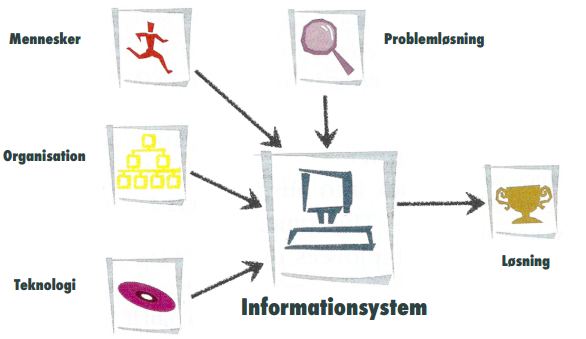
\includegraphics{images/kontekstmodel/metode.png}
  \caption[Metode for Kontekstmodellen]{Illustration af elementerne i et informationssystem. Kilde:
  \protect\citet{Laudon1999}}
  \label{fig:kontekstmodel}
\end{figure}


%\section{Informationssystem}\label{Informationssystem}
\subsection{Informationssystem}\label{subsec:Informationssystem}

Et informationssystem bruges til at effektivisere en arbejdsproces og hjælper med at holde fokus, så arbejdet
bliver gjort tilfredsstillende. Informationssystemet består af tre processor: Indsamling af data, behandling
af dataene og formidling af dataene. Der indsamles data om de tre elementer: mennesker, organisation og
teknologi. Når dataene er indsamlet, behandles de, altså der bliver analyseret på dataene. Herefter formidles
det i form af, der findes ud af, hvad datene kan bruges til. Behandlingen af de tre elementer bruges til at
finde ud af, hvad der skal tages hensyn til under problemløsningsdelen. Alt dette er et informationssystem,
som bruges til finde ud af, hvad løsningen til problemstillingen er.


%\subsection{Mennesker}\label{subsec:mennesker}
\subsubsection{Mennesker}\label{subsubsec:mennesker}

Elementet mennesker handler om personer/persongrupper, som har en interesse i, at en given problemstilling
løses. Det kan være brugeren af det program, der bliver lavet og andre, som får gavn af en løsning. Man
undersøger bl.a. brugerens evner, da programmet skal laves på en sådan måde, at brugeren har den
fornødne kunnen, til at kunne betjene programmet. Brugerens behov undersøges også, så man får alle de funktioner
med, som er nødvendige for at programmet er brugbart.


%\subsection{Organisation}\label{subsec:organisation}
\subsubsection{Organisation}\label{subsubsec:organisation}

Under organisationsafsnittet undersøges hvor og hvordan problemet opstår, derudover undersøges der hvilke regler
og værdier organisationen har, for at kunne tage disse med til problemløsningen.

\cbstart
%\subsection{Teknologi}\label{subsec:Teknologi}
\subsubsection{Teknologi}\label{subsubsec:Teknologi}

Teknologidelen omhandler de teknologier, som anvendes til at løse en informationssystem relevant problemstilling.
Ofte ville denne teknologi være en computere, servere, og internettet. Dette er altså de byggeblokke hvorpå
systemet bygges.
\cbend

%Teknologielementet handler om teknologier som allerede er på markedet, som kan løse problemstillingen. Dette
%behøver ikke kun at være løsninger som er computerbaserede, det kan også være manuelle systemer, altså hvor
%det hele gøres i hånden, med papir og blyant.


%\section{Rapportens opbygning}\label{sec:rapportens-opbygning}
\subsection{Rapportens opbygning}\label{subsec:rapportens-opbygning}

Først bliver menneskedelen behandlet, i form af en interessentanalyse, herefter vil organisationselementet blive berørt. Derefter bliver der skrevet om teknologier,
hvorefter de tre elementer munder ud i en problemafgrænsning og en problemformulering. Til sidst skrives der
om problemløsningsdelen. \fxnote{Sidste sætning skal udvides så der står hvad der vil blive skrevet om}


\part{Problemanalyse}

\chapter{Interessenter for en sejlklub}\label{chap:interessent-analyse-ved-sejlklubber}

I denne interessentanalyse, ses der på mennesker og grupper der har interesse i en specifik software løsning, konkret
til sejlklubber med sejlerskole. Der vil herudover blive set på hvad deres interesse er i projektet, samt hvilken
indflydelse en løsning ville kunne have på deres tilværelse.


Der vil for interessenternes vedkommende blive set på hvad, de hver især kunne få gavn af i henhold til projektet. 
Det er værd at notere at hver enkelte klub har forskellige behov, så dette er en generel forståelse af interessenternes
behov. Forståelsen for de forskellige grupper interessenter er dannet ud fra et Interview med tidligere skolechef på
Sundet. Interviewet kan findes i \myref{bilag:interview}.

\section{Interessenter for sejlklubbers administrative opgaver}

\subsection{Dansk sejlunion}

Dansk sejlunion er et forbund, som blev dannet i 1913, og har ikke nogen direkte grund til at være interesserede i
projektet.
Et af deres mål er som forbund at hjælpe sejlklubber med service, rådgivning mm. og derfor, menes det at Dansk sejlunion
også vil være interesseret i et system der vil kunne hjælpe de frivillige i deres arbejde.

Deres mission er at være det nationale samlingspunkt for alle sejlere. Dansk sejlunion er tilsluttet Danmarks
Idrætsforbund, International Sailing Federation og andre lignende organisationer inden for sejlsport.
\citep{Sejlsportdk}


\subsection{Medlemmer}

Hver sejlklub bestemmer selv deres opbygning organisatorisk af hvilke type medlemmer de har i klubben. Der vil blive
fortalt mere om dette i \myref{chap:organisation}. 

Medlemmerne i sejlklubben er de personer som bruger sejlklubbens faciliteter. Herudover også her klubben får deres
indtægter til at kunne holde sig i gang, og investere i eventuelt nye både el. \fxnote{Sidste sætning skal rettes men
kan ikke gennemskue hvad der rigtigt skal stå?} Det er derfor vigtigt at klubberne gør medlemmernes tid ved sejlklubben
så god som mulig. Et system der kunne hjælpe medlemmerne med at finde informationer, leje både, og som har
medlemmernes interesse i højsædet, vil helt klart kunne være i deres interesse. De førnævnte funktioner i et system til
en sejlklub, er netop funktioner der sandsynligvis ville blive brugt mest af medlemmer.

Medlemmer i en sejlklub kan være en meget bred gruppe fra den yngre befolkningsgruppe, til den noget ældre. Det er
derfor vigtigt at lave et design, som er intuitivt i anvendelse, for alle brugere. 

%Interessentgruppen ``medlemmer'' omhandler medlemmer af sejlklubber. Det er meget forskelligt fra sejlklub til
%sejlklub hvordan medlemmer kategoriseres eller om de overhovedet gøres dette. F.eks. så har ``Sejlklubben
%Sundet'' kategoriseret deres medlemmer således: Voksen-, Bådejer-, Gaste-, Mini-kølbåd-, Ungdoms-, Passiv- og
%Støttemedlem.
%[http://www.sundet.dk/vedtaegter/Vedtaegter%20for%20Sundet%2027nov12.pdf]

%Til sammenligning har Vestre Baadelaug kategoriseret deres medlemmer efter følgende: Aktive-, passive- og
%æresmedlemmer.
%[http://www.aalborglystbaadehavn.dk/UserFiles/file/VB_filer/Statiske_filer/Vedtaegter_2008-9_web.pdf].

%Fælles for medlemmerne er, at de gerne vil have informationer fra klubberne, så de ved hvilke begivenheder der finder
%%sted. Det kan være kapsejladser, foredrag, o.lign. Der er mange informationer, medlemmer fra en sejlklub kan modtage.
%\section{Gæster}:
%Gæster har ikke nogen primær funktion når det kommer til udlån, de bådklubber der tilbyder udlejning af både,
%%forbeholder denne funktion til medlemmer, som har bestået et førerkursus accepteret af den givne bådklub.


\subsection{Undervisere}

En sejlklub med sejlerskole, skal også have undervisere til sejlerskolen, og disse kan også drage nytte af et system til
at hjælpe med administrative opgaver. Underviserne vil ved hjælp af et system eventuelt kunne sende afbuds e-mails eller sms-beskeder ud til alle på
undervisningsholdet. Det vil muligvis kunne gøre det lettere for underviseren at holde styr på den enkelte elevs fremgang
ved undervisningen m.m. hvilket medfører at underviserne bør have andre funktioner i et system til en sejlklub end medlemmerne
ville have, de ville eventuelt kunne stå for at registrere hvem der har et førerbevis i klubben, ol. Underviserne kan også
være frivillige i sejlklubben, men de er beskrevet for sig selv da de har mere specifikke funktioner i sejlklubben. 
Det antages at hvis et system ville kunne hjælpe undervisere med deres opgaver, så de bruger mere af deres arbejdstid på
at undervise, ville det give en positiv respons.

\subsection{De frivillige i sejlklubben}

Der er udover undervisere i en sejlklub også andre frivillige der arbejder i sejlklubben. Dette kan være lige fra en
formand til en sekretær eller måske endda nogen som gør rent i sejlklubben. Disse frivillige kan alle have forskellig
gavn af et system, der kan håndtere deres anliggender i sejlklubben, og er derfor taget med som interessenter. Nogle af
dem kan have til opgave at holde styr på ind- og udbetalinger for medlemmerne, hvilket et medlemssystem ville kunne
hjælpe med. En sekretær ville kunne give nyheder eller referater videre til klubbens medlemmer igennem sådan et
system. Så der er altså mange forskellige muligheder et administrativt system ved en sejlklub ville kunne hjælpe med, og
herudover også mange mennesker der ville kunne få gavn af en løsning.


Disse 4 interessenter, har hver deres interesse for projektet, hvor underviserne og de andre frivillige smelter en smule
sammen. Underviserne samt de andre frivillige, vil gerne have det gjort lettere at udføre deres frivillige arbejde.
Medlemmerne vil gerne have informationer fra klubberne angående begivenheder der
måtte foregå, samt muligheder for at deltage i disse, eller leje sejlbåde.
Dansk Sejlunion er altså en mindre direkte interessent, men kan dog have interesse i at hjælpe nye eller mindre
sejlklubber med at istandsætte et godt administrativt netværk, for at danne en velfungerende sejlklub, 
der giver gode oplevelser for medlemmerne.


\chapter{Organisation}\label{chap:organisation}

\cbstart

\section{Sejlklubben Sundet}

I Sejlklubben Sundet findes flere både, af forskellig størrelse, som bruges til undervisning af klubbens
elever, såvel som udlån til klubbens medlemmer.

Undervisningen foregår hen over hverdagene, hvorimod bådudlån foregår i weekenderne. En enkelt klasse af både
kan dog også udlånes om onsdagen.

For at måtte sejle skal der være minimum én fører med i bådens besætning \fxnote{Husk at definere fører og
muligvis besætning, hvis dette bibeholdes.}. Desuden bestemmes prisen for udlånet bl.a. efter besætning også,
idet tilstedeværelsen af en af klubbens elever gør, at udlånet er gratis.

Håndteringen af de forskellige data blev, og bliver muligvis stadig, udført på papir, ved manuelt arbejde,
hvilket ifølge oplysninger \fxnote{Muligvis angive en mere officiel kilde her?} kan resultere i, at det kun
bliver gjort engang imellem.

Ved et kig på Sejlklubben Sundets hjemmeside \citep{SundetUdlaan} ses det, at forskellige værktøjer er taget i
brug, i et forsøg på at øge brugervenlighed og interaktion mellem deltagere. Det er på nuværende tidspunkt
uvist, hvor vidt disse tiltag har haft den ønskede, gavnlige effekt.

\cbend

\chapter{Teknologianalyse}\label{chap:teknologi-analyse}

I det følgende kapitel vil forskellige teknologier, som kunne anvendes i forhold til at hjælpe med
administrationen i en sejlklub, blive forklaret. Derefter findes en analyse af de programmer, som på nuværende
tidspunkt er state of the art inden for administration af sejlklubber.

\section{Teknologier}

\subsection{Internet}

En fordel for et system til administration i alle typer af klubber og organisationer ville være at kunne tilgå
det fra flere steder end bare et sted. Ved at gøre et system netværksbaseret kunne medlemmer og frivillige
tilgå det fra hjemmet, deres arbejdspladser eller måske endda deres mobile enheder, og derved ville en tur ned
til klubhuset, f.eks. for at undersøge om der var en båd ledig den kommende uge, undgås, hvilket der i
\myref{sec:organisation-konklusion} blev fremlagt som et problem. Anvendelsen af et system, som kunne operere
over internettet, kunne altså øge informationsspredning i klubben. Herved gøre det muligt at lave papirarbejde, som
udfyldelse af log-filer hjemmefra i stedet for i klubben og tilmelde sig sejladser og andre arrangementer
hjemmefra.


\subsection{Server}

For at alle medlemmer og frivillige arbejdere i en klub kan tilgå systemet over internettet, skal systemet
opretholdes af en server, hvorfra andre computere kan forbinde sig til og bruge systemet. En mulighed for
opsætning af en server ville være at få en computer i selve klubhuset til at agere server og have systemet, og
al information, til at ligge der. Dette er dog en dårlig løsning, da klubben selv skulle stå for opdatering af
serversoftware, tage backup af al data og det ville kræve mere af klubbens internetforbindelse. En anden
mulighed for at en klub ikke selv skulle stå med at administrere en server, er at købe sig ind hos et hosting
firma. Her kan man have systemet kørende på en server, og firmaet varetager samtidigt al vedligeholdelse af
server og serversoftware og sørger for backup af al data. Dog kan forskellige firmaer have forskellige måder
at gøre tingene på, men de firmaer der kigges på i de følgende afsnit, \textit{abakomp} og \textit{Softcom}, sørger begge for vedligholdelse og overvågning af serverne, og for at tage backup. 

De typer af servere, der bliver udbudt af hosting firmaer, kan deles op i dedikerede servere og i virtuelle
servere.


\subsubsection{Dedikerede servere}

Ved en dedikeret server lejer man hele maskinen, som skal køre systemet, og man får derfor mere ud af maskinen
og har mere indflydelse på komponenterne i maskinen og hvilket operativsystem der køres. En dedikeret server
ville umiddelbart være bedre for større klubber/organisationer, hvor mængden af informationer serveren skulle
kunne håndtere er større og trafikken til serveren også ville være højere. \citep{Dedikeretserver}


\subsubsection{Virtuelle servere}

Alternativet til at leje en hel maskine til at køre et system, er at leje en virtuel server, hvor der på den
samme fysiske maskine findes flere separate virtuelle servere. At leje en virtuel serverplads er billigere end
at leje en dedikeret server, da en virtuel serverplads kan lejes for helt ned til 850 kr. i
måneden\citep{Virtuelserver}, hvorimod en dedikeret server kan lejes fra 1062 kr. i måneden
\citep{Dedikeretserver}. 
Dog variere prisen alt efter hvilket hardware der bruges og efter, hvor meget
serverplads man ønsker. Grunden til at en virtuel serverplads er billigere, er at flere forskellige virtuelle
servere kan køre på samme fysiske maskine, og derved er der flere til at betale for vedligeholdelsen. Men en
virtuel server har til gengæld ikke lige så meget plads og kraft som en dedikeret server.

En virtuel serverplads ville umiddelbart være nok til at køre et administrativt system for en sejlklub, og det
ville desuden være billigt at leje plads hos et hosting firma. Det er derfor fornuftigt at antage at
sejlklubber har midler til at leje en serverplads, hvilket ville kunne anvendes til at køre et administrativt
system med alle informationer, som kunne være nødvendigt for systemet.


\subsection{Brugergrænseflade}

I et program som skal anvendes af en bruger eller brugergruppe, ønskes det, at programmet har et udseende, som
brugeren forstår og som hjælper med at bruge programmet. Her menes der programmets interface, på dansk,
brugergrænsefladen. Det er vigtigt, at brugergrænsefladen henvender sig til modtagergruppen, hvilket i dette
projekt er personer med tilknytning til en sejlklub. Der skal desuden tages højde for de forskelle i teknisk
snilde, der er i modtagergruppen, da det ikke er effektivt at lave et system, som halvdelen af modtagerne ikke
kan bruge. Forskellige undergrupper i modtagergruppen skal bruge forskellige funktioner i systemet, og derfor
skal interfacet tilpasses, så de korrekte funktioner bliver tilgængelige for de rigtige brugere.

En mulighed for at skabe en brugergrænseflade i samarbejde med C\#-kode, er ved at anvende \textit{Windows
Forms}. Det findes også andre muligheder for at anvende C\#-kode til at skabe brugergrænseflader som
\ac{MVC} og \ac{WPF}, men i løsningsdelen vil
\textit{Windows Forms} blive anvendt til at skabe en brugergrænseflade.

\subsection{Management systemer}\label{subsec:management-systemer}

Et system som med fordel kunne anvendes til det formål, er et management system. Et management system er et
framework af processer og procedurer, som bruges til administration af frivillige organisationer og
virksomheder. Eksempler på management systemer findes i \myref{chap:teknologi-analyse}. Mere præcist er
SailingClubManager et management system, hvilket er yderligere dokumenteret i \myref{bilag:scm}. Det
management system har en \ac{GUI} i web browseren. Dette er i kontrast til en konsol
applikation, eller en nativ \ac{GUI}.

Ved at anvende et management system kan en klub eller forening, forudsat at systemet er succesfuldt, mindske den
tid, der bruges på papirarbejde. Særligt fordi en lang række idrætsforeninger drives af frivillige. Ifølge
\citet{Frivilligrapporten} er 26\% af de arbejdsopgaver, som findes for frivillige, sekretariatsarbejde og
administrativt arbejde. Med et godt management system kan de administrative opgaver derved bringes ned på
mindre tid, og derved kan de frivillige bruge deres tid på mere interessante ting for organisationen, eller
bruge den ekstra tid på noget andet.


\section{State of the art}

For at kunne udvikle et godt produkt, der skal kunne bruges i en bådklub, er det vigtigt, at se på hvilke
produkter der allerede er på markedet, altså hvad er ``state of the art''. I denne forbindelse er der fundet
forskellige produkter, som har nogle af de features der efterspørges i et system til en bådklub.


\subsection*{BoatCloud}

Der er f.eks. et program udviklet af Anderson Software, der hedder BoatCloud.\citep{BoatCloud} BoatCloud
består af 3 applikationer, StackTrack, VesselValet og Service Request. StackTrack benyttes, når medlemmerne selv sejler
deres både, hvorimod VesselValet, er
når der skal tjenere og passagerer med ombord på bådene. BoatCloud applikationerne er derfor mere designet til
en bådklub, som passer på medlemmernes både, fremfor klubbens egne både. I applikationerne kan medlemmerne
melde, at de vil sejle på et bestemt tidspunkt. Medlemmet kan få klubben til at vaske båden, tanke den, og
fylde den op med diverse snacks, alt sammen registreres igennem denne webbaserede applikation. Applikationen
tager imod alle disse bestillinger i realtime, og 24 timer i døgnet. Herudover bliver der sendt e-mails ud til
medlemmerne, når de har lavet en bestilling. Man kan logge ind som administrator, og her kan man se alle
reservationer, der er lavet, samt have mulighed for at se yderligere detaljer om hver enkelt reservation.


\subsection*{Sailing Club Manager}

En anden applikation der findes er Sailing Club Manager \citep{SailClub}. Denne applikation er også
webbaseret, og gør det muligt for en bådklub at tilføje hvilke både der er, samt hvor det er fortøjet i
havnen. Man kan i en kalender lave begivenheder og reservationer, samt medlemstilmeldelse til forskellige
begivenheder. Applikationen kan også bruges som kontaktmedium for klubben til deres medlemmer. Klubben kan
sætte et e-mail system op, samt tilføje et template som bliver sendt med hver enkelt e-mail. Applikationen kan
endvidere holde styr på økonomien, man kan tilføje en bankkonto, samt  holde styr på fakturaer, og endda sende
dem og håndtere det online. Man kan tilføje medlemsskaber, med forskellige oplysninger omkring medlemmerne der
har netop dette medlemsskab i klubben.



Ud fra denne undersøgelse er flg. features altså fundet i applikationerne:

\begin{itemize}
  \item Medlemmer kan reservere afgange
  \item Medlemmer kan melde sig på begivenheder i bådklubben
  \item Medlemmer kan betale igennem hjemmesiden
  \item Medlemmerne kan bede klubben om at gøre deres egen båd klar, med forskellige aftaler klubben håndterer
        før den aftalte tid
  \item Bådklubben kan vise hvilke både der er i klubben
  \item Bådklubben kan oprette begivenheder, og afsætte hvilke medlemmer der kan melde sig på begivenheden
  \item Bådklubben kan oprette forskellige medlemsskaber og opkræve betalinger igennem hjemmesiden
  \item Bådklubben kan sende e-mails med klubbens egen template gennem hjemmesiden, herunder påmindelser om en
        reservation nogen tid før.
\end{itemize}

I bilag \myref{bilag:scm} findes der screenshots af udvalgte features der findes i SailingClubManger.

\subsection*{ForeningLet}

ForeningLet er en applikation, som adskiller sig fra de andre ved ikke at henvende sig specifikt til én type klub, desuden er det en dansk applikation. Applikationen er web-baseret og har mange nyttige funktioner for en sejlklub som Sundet. Applikationen har en medlemsdatabase, et regnskabssystem samt en kontaktfunktion som kan benytte både e-mail og SMS. Der kan også opkræves betalinger fra medlemmerne gennem systemet. Applikationen har også en reservationsfunktioner. Desuden kan der oprettes begivenheder i applikationen, som medlemmerne også kan tilmelde sig gennem applikationen. ForeningLet giver også foreningen mulighed for at oprette deres egen hjemmeside samt deres egen online butik. 


\section{Konklusion af teknologianalyse}

Ud fra teknologianalysen er de teknologiske aspekter i projektet blevet belyst. Muligheden for at gøre
systemet netværksbaseret, gør det muligt for medlemmerne og administrationen i en sejlklub, at foretage
handlinger vedrørende klubben fra hjemmet eller arbejdspladsen. For at undgå at en lokal server skulle
opsættes og vedligeholdes af klubben selv, kunne en virtuel server, hostet af et hosting firma, varetage denne
opgave. Vigtigheden i en god brugergrænseflade blev gjort klart, og metode for at opsætte en brugergrænseflade
blev valgt i form af \textit{Windows forms}. Fra state of the art delen blev nuværende systemer på markedet
undersøgt, og udvalgte features tages med videre til løsningsdelen, som eventuelle tilføjelser til det
administrationssystem der skal udvikles.



\input{chapters/management_systemer.tex}
\chapter{Problemformulering}\label{chap:problemformulering-new}

Indtil nu er problemet om fritidsklubbers administrative opgaver blevet belyst og analyseret vha. Laudon og Laudons model beskrevet i \myref{chap:struktur-af-problemanalyse}. 
Det er nu ud fra denne analyse muligt at komme frem til en problemformulering, som der vil arbejdes ud fra i løsningsdelen henimod en løsning til fritidsklubber og ikke mindst sejlklubber.

Der blev i \myref{chap:Fritidsklubber}, omhandlende fritidsklubber, afgrænset til sejlklubber, da disse viste sig at have flere specifikke administrative opgaver, sammenlignet med andre fritidsklubber. 
Denne afgrænsning blev foretaget da et system, der kan håndtere generelle samt specifikke opgaver til en sejlklub, kan bruges af andre former for fritidsklubber ved at tilpasse specifikke funktioner.
Ved at analysere videre på de direkte forhold vedrørende en sejlklub, blev der dannet en forståelse for, hvilke problemer en sejlklub med sejlerskole har, som kan løses vha. et administrations system.


\section{Interessenterne for sejlklubber}

Der var forskellige interessenter for sejlklubberne, og de havde varierende mængder af interesse i projektet.

Medlemmerne, underviserne og de frivillige vil alle være personer der skal bruge det udviklede system. 
De har derfor en mere direkte indvirkning på, hvordan system skal opbygges. 
Hvis systemet ikke har de funktioner, som de efterspørger, vil det ikke være den gode løsning, som de gerne vil have. 
Dette gælder for alle de tre nævnte interessenter. 
Det skal dog understreges, at de ikke vil bruge samme dele af systemet. 
Dette skyldes, at medlemmerne ikke skal kunne oprette undervisningsdage mm., da det kun er underviserne, der skal have tilladelse til dette. 

\section{Organisation}

I forbindelse med organisationsafsnittet blev der undersøgt, hvordan sejlklubberne håndterer forskellige opgaver i klubben, samt hvilke opgaver de beskæftiger sig med.

Det viste sig, at klubberne har individuelle medlemstyper, og det kan derfor være relevant at lade klubberne selv oprette forskellige medlemstyper i systemet. 
Desuden efterspørges det, at man kan tilkoble sig systemet hjemmefra, for således at kunne få informationer om begivenheder og undervisning i klubben, og måske endda tilmelde sig disse, uden at tage turen ned til klubben.

Grundet den store mængde af information, der skal nedskrives, i forbindelse med en sejlads, giver det mening at hjælpe med at organisere denne opgave, samt at gøre det lettere at registrere informationerne for diverse frivillige og undervisere. 
Desuden kunne det hjælpe hvis hvert medlem havde en saldo over udgifter ved sejlklubben, således det er nemmere at håndtere brugerbetaling.

Følgende er en liste over opgaver, som kan dækkes af et system for sejlklubberne:

\begin{itemize}
  \item Tilkobling hjemmefra, via internettet
  \item Mulighed for at få informationer vedr. begivenheder, samt at tilmelde sig disse
  \item Organisering af information der nedskrives i forbindelse med en sejlads
  \item Organisering af betalinger, samlet for det enkelte medlem, samt mulighed for online betaling
  \item Booking af både
  \item Administrering af undervisning
\end{itemize}


\section{Teknologi}

Sejlklubben Sundet, viste sig at have flere forhold at organisere end de andre klubber der er undersøgt, og derfor afgrænses projektet til konkret at designe et IT-system til Sundet. 
Dette gøres da hvis et system kan hjælpe Sundet, er det blevet konkluderet, at det også kan hjælpe andre sejlklubber, der har færre forhold at holde styr på.
Man har fundet frem til at systemet, der efterspørges, er af typen management system, som blev beskrevet i \myref{subsec:management-systemer}.
Der findes allerede systemer, som kan dække Sundets administrative behov, bortset fra håndteringen af undervisning.
Der mangler altså et program på markedet, som kan håndtere en sejlklubs sejlerskole.
Heri ligger projektets eksistensberettigelse.

\subsection*{Problemformulering}
\subsubsection*{Ud fra denne afgrænsning er flg. problemformulering formuleret:}

\begin{center}
  \begin{tabular}{|p{14cm}|}
    \textit{Det er et problem at frivillige i fritidsklubber med specielle udlejningsmuligheder, så som Sundet, benytter unødvendig arbejdskraft på fysisk dokumenthåndtering vedrørende udlånte faciliteter, undervisning og begivenhedsorganisation. 
    Hvordan kan et system hjælpe med at danne overblik over sådanne opgaver?}
  \end{tabular}
\end{center}
\fxnote{Nikolaj: bør det ikke nærmere være: "Hvordan kan der udvikles et system som kan hjælpe med at danne overblik over sådanne opgaver?}


\section{Afgrænsning for problemløsning}

Da dette projekt er udarbejdet i løbet af 2. semester på Aalborg Universitet, er der ikke uanede mængder af tid. 
Der afgrænses derfor fra at udvikle hele management systemet til sejlklubben Sundet, til i stedet at lave enkelte dele af systemet.

Grundet de manglende ressourcer og tid, vil der altså ikke blive lavet et system, der kører over internettet, men i stedet et system, som kan håndtere de forskellige emner lokalt. 
Denne afgrænsning finder sted, da hvis funktionerne for klubben kan fungerer på computeren, skal det tilkobles en server, for at kunne tilgåes fra flere forskellige computere. \fxnote{Hvad menes der med ``computeren'' er det den nede i klubben, eller enhver?}
Derfor ser projektgruppen altså funktionerne for Sejlklubben Sundet som værende de vigtige ting at udvikle, selvom systemet mister noget af sin effektivitet uden internetopkoblingen.\fxnote{Nikolaj: Omformulering: " selvom systemet mister sin brugbarhed uden internetopkoblingen}
Men dette ses som værende acceptabelt, da systemet ikke skal tages i brug af klubben, da dette er et projekt lavet i forbindelse med uddannelsen på Softwareingeniørstudiet ved Aalborg Universitet.

De resterende kapitler i rapporten, vil beskæftige sig med udviklingen af et management system, henvendt imod Sejlklubben Sundet, baseret på problemformuleringen. 
Som det første vil der komme en kravspecifikation for systemet, på baggrund af denne afgrænsning.

\chapter{Produktkrav}

Igennem problemanalysen blev det gjort klart, at der findes et problem ved fritidsklubber, særligt Sejlklubben Sundet, når det kommer til management af deres ressourcer samt dokumenthåndtering. 
Problemet kan løses ved et management system, til at håndtere dokumentation for sejlklubben og gøre det overskueligt. 
I følgende afsnit undersøges der, hvilke krav et managements system for Sejlklubben Sundet skal have. 


\section{Funktionelle krav} \label{sec:funktionelleKrav}

Den nødvendige dokumentation indebærer logbøger, bådreservationer, besætningslisten, tilmeldinger til begivenheder m.m. 
Som grundlag for at alt dette kan fungere, kræves der en metode til at sætte sig selv på en aktivitet. 
For at gøre dette muligt kræves der således to ting: En database af medlemmer, samt en form for begivenhedskalender. 
Foruden dette kræves der information om de forskellige begivenheder og hvem der er tilmeldt. 
Der kræves også et system til udlejning af både samt undervisning.

Produktet bør have følgende funktioner i prioriteret rækkefølge:
\begin{itemize}
  \item Medlemshåndtering
  \item Brugerlogin
  \item Oversigt over undervisning
  \item Bådreservation
  \item Logbog
  \item Vise begivenhedsinformation
\end{itemize}


%Dette afsnit skal uddybes meget mere, har skrevet et eksempel på hvad jeg mener afsnittet skal indeholde

\section{Uddybning af funktionelle krav}

Der ligger mere bag de ovenstående elementer end \myref{sec:funktionelleKrav} giver udtryk for, disse vil her blive set nærmere på.

\subsection{Medlemmer}

Det er et krav at man kan udnytte medlemmerne i klubben, så man kan registrere hvem der er tilmeldt de forskellige reservationer eller lignende. 
Systemet skal kunne kende forskel på medlemmer, så man ikke kan have flere af det samme medlem på en reservation eller en begivenhed.
Forskellige informationer skal kunne findes på medlemmerne i programmet, så brugerne kan finde de rigtige medlemmer og markere om de mødte op.

\subsection{Login system}
Det skal være muligt at registrere hvem der er logget ind i programmet, for på denne måde at give forskellig adgang til diverse funktionaliteter i programmet.

\subsection{Oversigt over undervisning}

Det skal være muligt for elever ved sejlerskolen at se hvornår deres næste lektion finder sted.
Herudover skal de også kunne se hvor langt de er kommet i forbindelse med deres uddannelse. Hvilke milepæle de har udført, mm.
Underviserne skal have mulighed for at oprette nye lektioner og angive hvilke læremål eleverne udførte i den pågældende lektion. 
Underviserne skal også kunne udforme og redigere hold på skolen hvis nogle skulle melde sig ud, eller ved sæsonstart.

\subsection{Bådreservation}

Medlemmerne i klubben har muligheden for at reservere klubbens både, og skal derfor kunne gøre dette i programmet.
Derfor skal der være en måde hvorpå man kan tjekke om en båd er booket i en given tidsperiode, og samtidig en måde hvorpå man kan reservere båden.
Herudover skal det være muligt af afmelde sig en booking hvis man ikke deltager alligevel, og dermed åbne op for nye besætningsmedlemmer.


\subsection{Logbog}

I forbindelse med en sejltur, skal der kunne gemmes en logbog over turen med informationer, som beskrevet i \myref{subsec:bådudlån}.
Der skal her være registreret på hvilken både turen foregik, så de korrekte logbøger kan findes for en given bog.

\subsection{Vise begivenhedsinformation}

Endeligt skal man kunne gemme begivenheder i klubben, med en dato og en beskrivelse af begivenheden. 
Det skal være muligt at til- og afmelde sig begivenheden, foruden at kunne se hvilke medlemmer der er tilmeldt.
Desuden skal der kunne vise en liste over begivenheder sorteret efter dato, så man kan danne et overblik over hvornår der sker hvad i klubben.


%\part{Problemløsning}

%\chapter{Eksempler}

{\itshape Dette dokument er primært ment som en hjælp til at se de forskellige muligheder
i rapporten.}

\section{Akronymer}
For lettere at håndtere akronymer, benyttes en pakke, hvor disse defineres én gang, og bruges så i
dokumentet ved hjælp af \textbackslash ac{acronym}. Så vil systemet sørge for, at skrive det fuldt
ud første gang man eksempelvis skriver \ac{AAU} eller \ac{KOT}.

Skulle det derefter ske, at man har behov for at snakke om \ac{AAU} igen, vil den bruge forkortelsen,
og dermed selv holde styr på det. Dette sikrer os bedre mod fejl. :)

\section{Ændringsregistreringer}
For at lette kommunikation med vejleder kan vi registrere ændringer på forskellige måder.

\subsection{Hele afsnit}
\cbstart Man kan markere, at et helt afsnit er blevet ændret eller tilføjet, ved hjælp af kommandoerne
\textbackslash cbstart og \textbackslash cbend, som markerer henholdsvist start og slut på sidebaren.\cbend

Det er også muligt at markere, at noget er blevet slettet, med \textbackslash cbdelete, hvilket er gjort i
dette \cbdelete afsnit.

\subsection{Detaljerede ændringer}
Der er også mulighed for at vise mere detaljerede ændringer. Eksempelvis \added[id=TB]{hvis man tilføjer tekst},
eller \deleted[id=TB]{sletter tekst}. Eller for den sags skyld \replaced[id=TB]{en kombination af de to}{a
combination of the two}.

\section{Matematik}
Matematiske formler er lette at indsætte\ldots

\begin{equation} \label{eq:example}
  f\left(x\right) = \dfrac{a \cdot b}{c}
\end{equation}

\section{ToDo--typer}
Der er fire forskellige typer af noter, og brugen heraf bestemmes af gruppen i fællesskab, så der er enighed om,
hvad der benyttes til hvilket.

\subsection{Generelt}
Først og fremmest er der noterne almindelig\fxnote{Peger på et bestemt sted i teksten.}
og \fxnote*{Fremhæver et tekststykke også.}{med modtagertekst}.

Ligeledes er der advarsler\fxwarning{Dette er en advarsel!} og fejl\fxerror{Dette er en fejl!}. Sidstnævnte
vil desuden forhindre dokumentet i at kompilere, hvis det markeres som værende \emph{final}.

Disse tre typer kan naturligvis også bruges i \emph{stjerneformen}, til at fremhæve et bestemt stykke
tekst som denne tilknyttes.

\subsection{Avanceret}
Til de lidt mere krævende noter kan det være nødvendigt med mere tekst, hvilket kræver et environment.

\begin{anfxnote}{Dette er en opsummering.}
Dette kan benyttes til at få nogle længere noter ind i teksten, hvis der eksempelvis er noget der skal
overvejes, hvor det bare ikke er nok men en lille notits.

Foruden denne anfxnote er der også \emph{anfxwarning}, \emph{anfxerror} og \emph{anfxfatal}, ligesom ovenfor.
\end{anfxnote}


\section{Referencer}
Det er muligt at referere til forskellige ting, eksempelvis kan nævnes \myref{eq:example}.

For at oprette en såkaldt \emph{label}, som senere kan refereres til, benyttes \verb|\label{key}|. Det er god
stil indenfor \LaTeX at benytte prefixes til de forskellige labels, eksempelvis:
\begin{table}[h]
  \begin{center}
    \begin{tabular}{ll}
      \toprule[1.5pt]
      \texttt{chap:}   & chapter              \\ 
      \texttt{sec:}    & section              \\ 
      \texttt{subsec:} & subsection           \\ 
      \texttt{fig:}    & figure               \\ 
      \texttt{tab:}    & table                \\ 
      \texttt{eq:}     & equation             \\ 
      \texttt{lst:}    & code listing         \\ 
      \texttt{itm:}    & enumerated list item \\ 
      \texttt{ex:}     & example              \\
      \bottomrule[1.5pt]
    \end{tabular}
  \end{center}
  \caption{Reference prefixes} \label{tab:reference_prefixes}
\end{table}


\section{Eksempelbokse}

\begin{example}{Overskrift}
  \label{ex:an_example}
  \lipsum[1]
\end{example}



\section{Programmeringskode}




%%%%%%%%%%%%%%%%
%% REFERENCES %%
%%%%%%%%%%%%%%%%

%\backmatter
\makeatletter\@openrightfalse
\let\cleardoublepage\clearpage
\part{Referencer}

%%% Bibliography %%%
\bibliography{bibtex/litteratur}

%%% Figures %%%
\newpage
\listoffigures

%%% Tables %%%
\listoftables


\@openrighttrue\makeatother


%%%%%%%%%%%%%%
%% APPENDIX %%
%%%%%%%%%%%%%%

\part{Appendiks}
\appendix
\settocdepth{chapter}
\chapter{Informationer påkrævet af sejlklubben Sundet}\label{bilag:sundet}

\section{Data på sejlladser og medlemmer}

Dette bilag har til formål at beskrive de information Sundet påkræver af de sejlere der sejler fra deres klub. Herudover er der også informationer omkring hvilke informationer sejlerskolen Sundet skal bruge på deres elever for at kunne lade dem bestå.

Når en skolesejllads skal foretages skal følgende informationer skrives ned skoleprotokollen:

\begin{itemize}
	\item Navne på læren og eleverne
	\item Ugedag
	\item Dato
	\item Fremmøde, i form af X for mødt, A for afbud
	\item Navne på gæster
	\item Afgang og ankomsttider
	\item Vind forhold
	\item Evt. Kommentarer, normalt henvisninger til skadesrapporterne, hvis sådanne er opstået
\end{itemize}

Alle disse informationer skrives for hver skolegang, og arkiveres i klubhuset, dvs. det er ikke elektronisk.

Når der sejles uden for skolen, dvs. fornøjelsesture, eller kapsejladser skal lignende information udfyldes, dog med visse ændringer:

\begin{itemize}
	\item Bådnavn/id
	\item Navn, telefonnummer for føren af båden
	\item Navne på alle i besætningen, evt. telefonnummer
	\item Startid og dato
	\item Forventet ankomstdato og tid
	\item Formål med turen, med indikation af område for sejladsen
	\item Reelle ankomstdato og tid
	\item Vind og vejrforhold
	\item Kommentarer
\end{itemize}

Hvis der sker skader på en båd under en sejllads skrives disse ned i skadesrapporten. Føren skal også læse op i denne bog før en sejllads for at sikre at man er klar over evt. skader på båden, som man skal være klar over. I denne bog skrives flg. oplysninger:

\begin{itemize}
	\item Dato
	\item Tekst der beskriver uheldet, eller skaden
	\item Her kan også skrives evt. svar fra bådchefen(Personen der sørger for båden)
\end{itemize}

Til at holde styr på medlemmernes oplysninger, bruger Sundet et Microsoft Access baseret system. Her er der personlige oplysninger på eleverne og medlemmerne, samt kan der printes girokort ud til håndtering af kontingenterne. Det bruges også til at holde styr på bådene i havnen som er ejet af nogle af klubbens medlemmer, samt deres lokationer. Dette system kan kun tilkobles lokalt på computeren lokaliseret i klubhuset.

\section{Informationer og andre events}

Når Sundet skal give informationer ud til medlemmerne, sættes disse op på en opslagstavle. Disse informationer kan f.eks. være tilmeldinger til diverse begivenheder såsom 24-timers sejladser eller onsdagsmatcher. Dvs. for at kunne tilmelde sig begivenheder i klubben skal man skrive sig på det bestemte tilmeldingsskema man finder i klubhuset. Det er ikke sikkert at medlemmer har tid eller når at opdage tilmeldingsfristerne på diverse begivenheder, hvilket kan resultere i et lavere fremmøde, og mindre aktivitet i klubben.

\chapter{Screenshots af SailingClubManager}\label{bilag:scm}

Dette bilag har til formål at underbygge afsnittet "\nameref{chap:teknologi-analyse}  (\ref{chap:teknologi-analyse})". Dette er et system, til administration af både, som vi har fået tilladelse til at prøve af skaberen. Siden hedder SailingClubManager, og er placeret på url'en \href{http://abs.boxstuff.net}{\textit{http://abs.boxstuff.net}}, "abs"\ da vores klub derunder hedder "Aalborg Boat Squad". Det er også muligt at anvende denne service til at lave sin egen hjemmeside til offentligheden, et eksempel på dette er: \href{http://www.thamessailingclub.co.uk/}{\textit{Thames Sailing Club}}.

\begin{figure}
	Siden /boats indholder de både, som er tilføjet af brugeren. \newline
	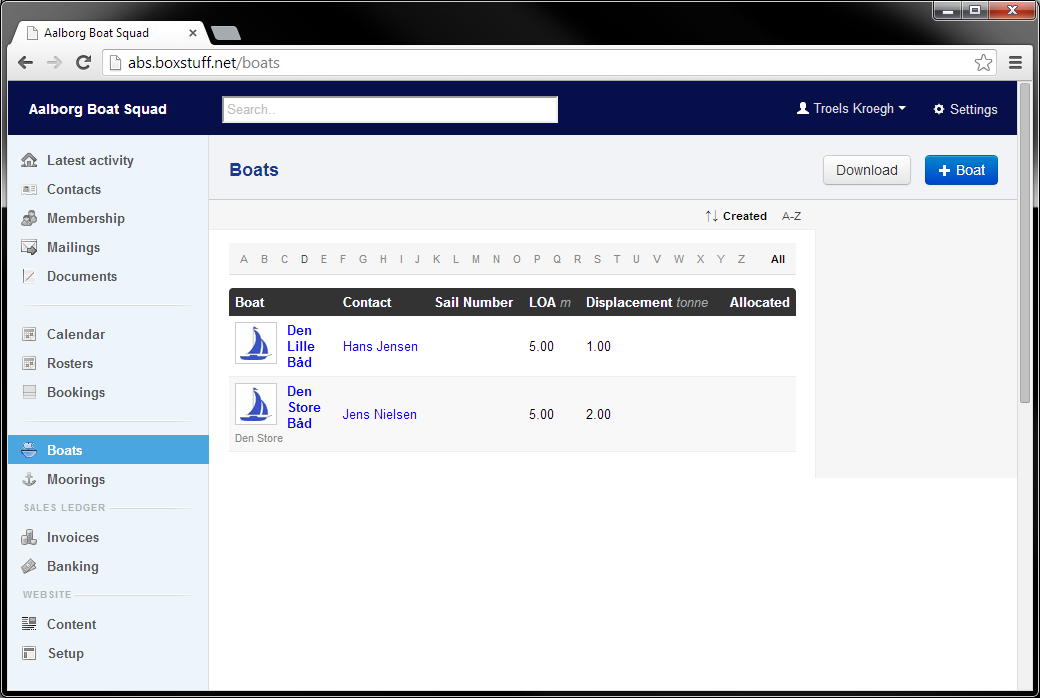
\includegraphics[scale=0.5]{images/teknologi/_Boats}
\end{figure}

\begin{figure}
	Personer som er en del af systemet, er en kontakt. De findes under /contacts.\newline
	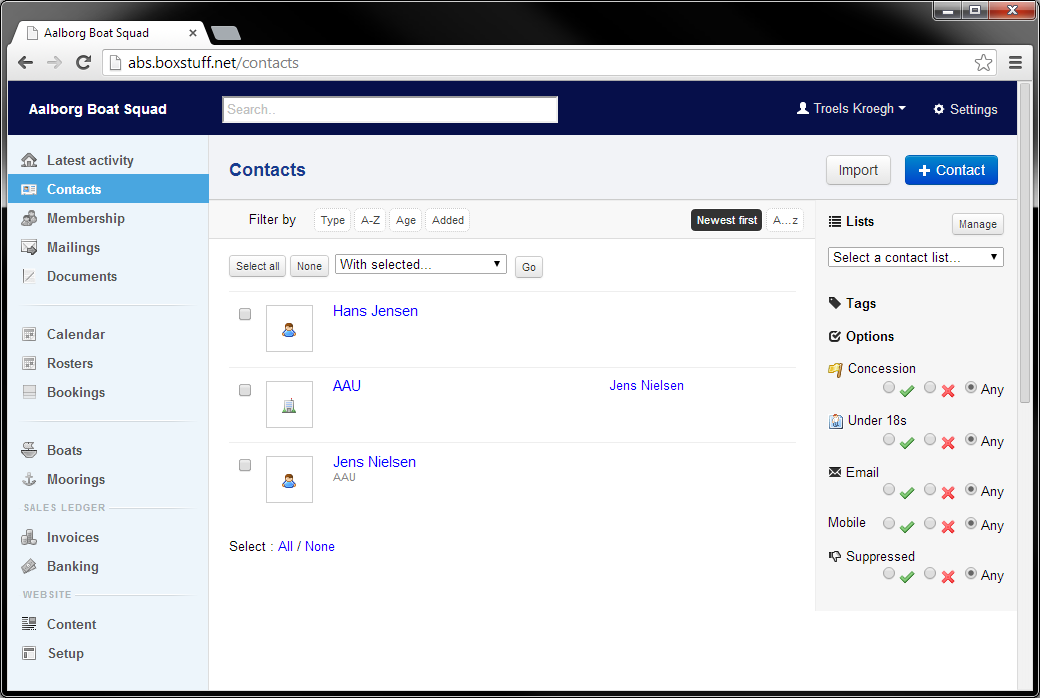
\includegraphics[scale=0.5]{images/teknologi/_Contacts}
\end{figure}

\begin{figure}
	Det er muligt at tilføje nye medlemmer, herunder hvilke type medlem de er. Disse typer er også muligt selv at lave i undermenuen Membership under /memberships/new.\newline
	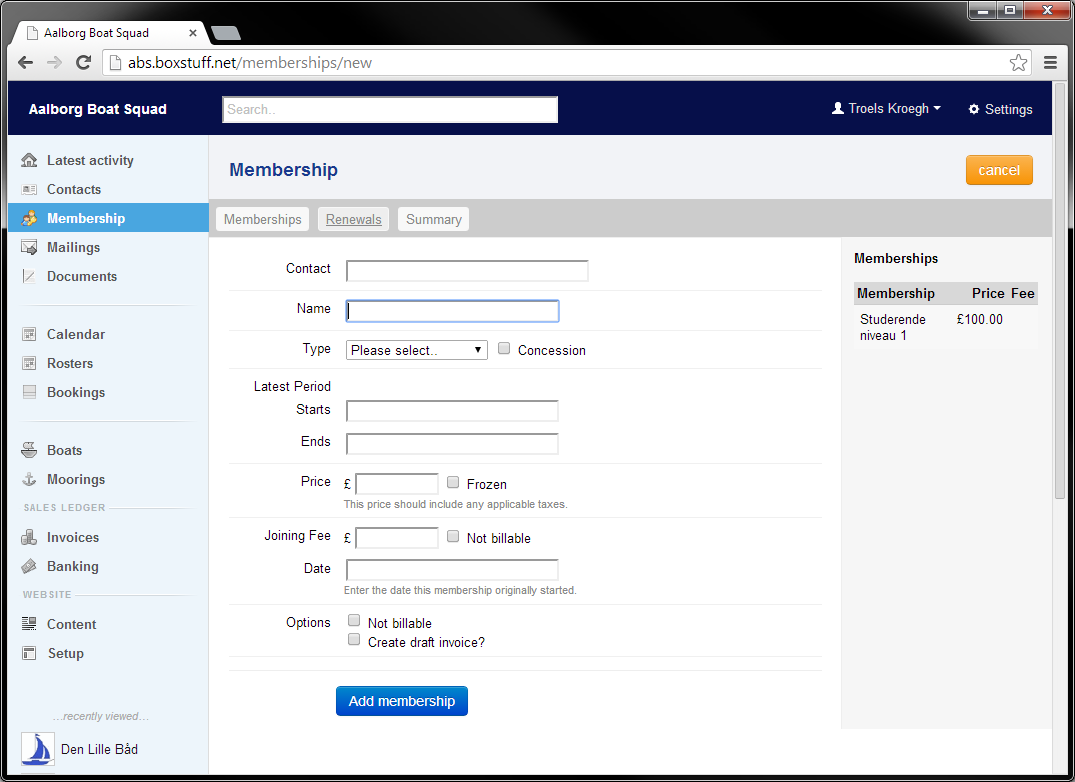
\includegraphics[scale=0.5]{images/teknologi/_AddMember}
\end{figure}

\begin{figure}
	Der findes en kalender med aktiviteter, som administratorer kan tilføje. Under /events.\newline
	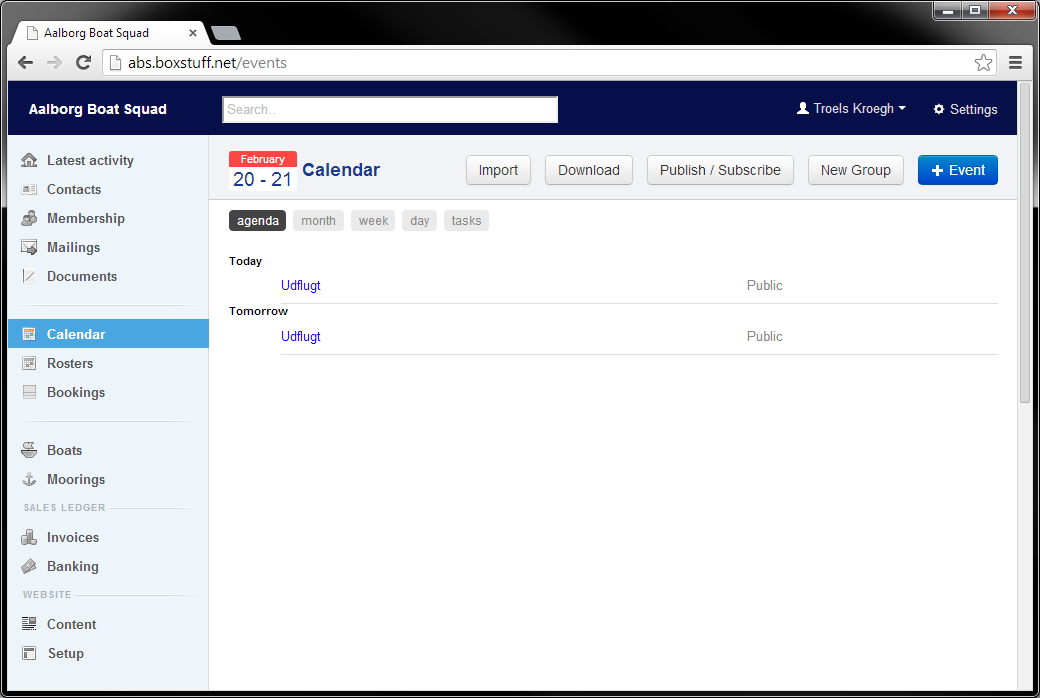
\includegraphics[scale=0.5]{images/teknologi/_Calendar}
\end{figure}

\begin{figure}
	Det er muligt for brugere at booke bådene, her har Hans Jensen booket en båd både den 20-02-2014 og den 26-02-2014. Dette findes under /booking/bookings.\newline
	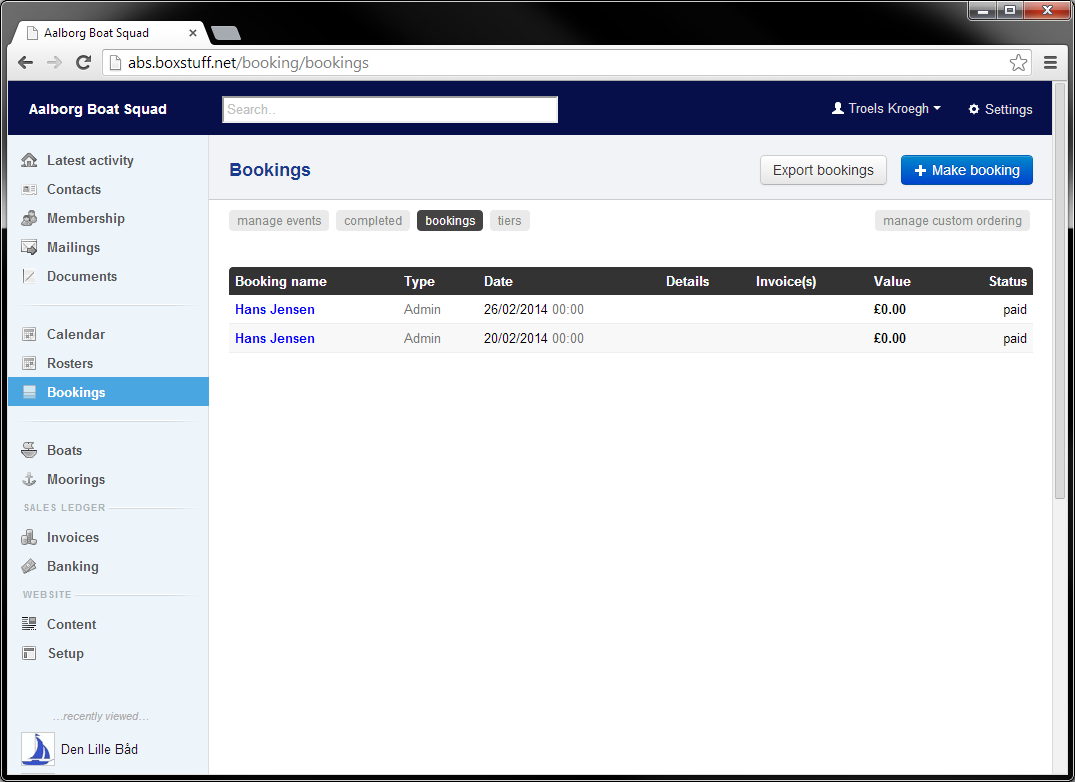
\includegraphics[scale=0.5]{images/teknologi/_Bookings}
\end{figure}

\begin{figure}
	Det er muligt at udskrive regninger baseret på brugeres udlån og kontingent. Under /invoices.\newline
	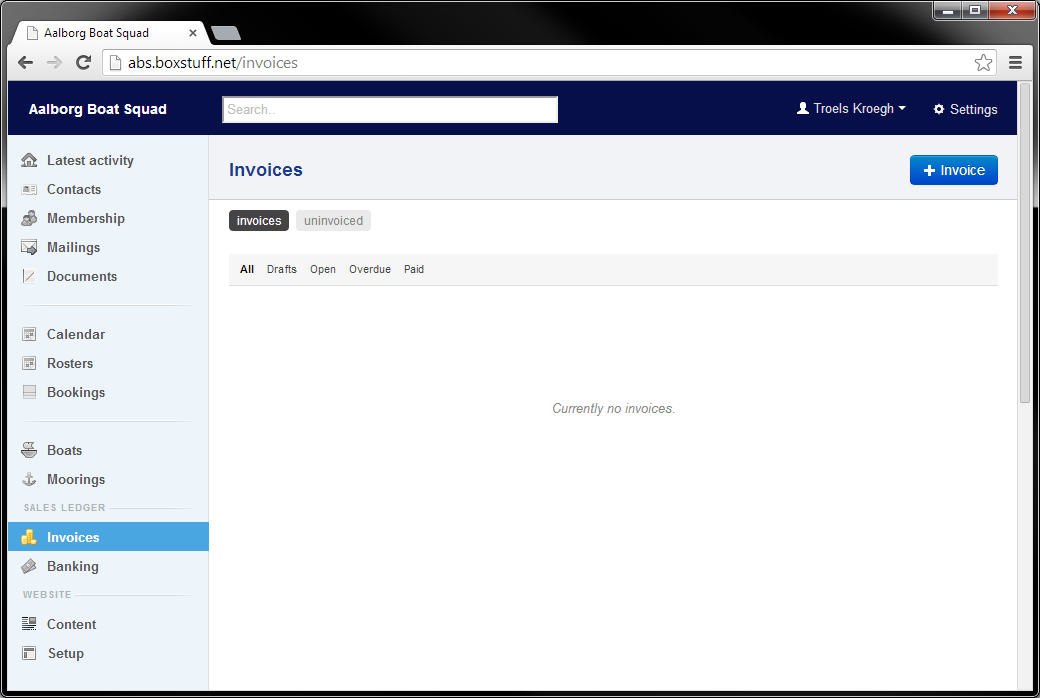
\includegraphics[scale=0.5]{images/teknologi/_Invoices}
\end{figure}

\chapter{Interview}\label{interview}
P- Peter Hinrup
D- Dorthe
K- Kasper
M- Mikkel
M2- Martin

P(00.00): der er 4 havne i aalborg hvor kommunen ejer havnen, hvor klubberne lejer havnen gratis imod at de selv vedligeholder den. Det er typisk en bådklub pr havn, ud over det bliver havnene nogle gange benyttet af andre mindre klubber så som kajakhavne eller søspejdere.

P(02.19): Der er 4 store havne i Aalborg, den her, Skudehavn, Marinafjordparken (aalborg sejlklub) og Nørresundby. De er ejet af Aalborg kommune imod at klubberne selv står for vedligeholdesen.

P(03.35): Vi er en forening med medlemmer som er medlemmer fordi de ejer en båd, hvorimod i Nibe kan man leje en plads, trods man ikke er medlem. I VB kan man ikke have en bådplads unden at være medlem.

P+D(05.00) viser gruppen en brochure med et kort over havnen.

P(06.25) Til sammen har VB og SL omkring 450 bådpladser, og i VB har de omkring 380 medlemmer og SL har omkring 150 medlemmer. I VB er det et familie medlemsskab, hvilket vil sige 1 båd = 1 medlem. 

D(07.31) Vores medlemskaber (SL) 	er pr hovede samt aktive og passive medlemmer.

P(08.00) Et medlem kan kun have en båd, dog i praksis ses det igennem fingrene, fordi det henner at et medlem køber en båd, også skal de have den gamle solgt. Det løses ved at et andet familiemedlem køber et edlemsskab

P(09.20) Dog sker det modsatte hvor der er flere ejere på en båd. Det er ofte unge mennesker der slår sig sammen omkring båden, men de skal alle være medlemmer, hvilket der ikke bliver tjekket op på.

D(11.40) SL og VB deler vandpladsen og betaler hver for sig leje til ANF. SL's medlemmer afregner pr kvadratmeter båd, hvorimod i VB, hvor de afregner pr pladskvadratmeter. Alle både beholder eller får nye pladser til foråret. Men man kan ikke købe en permanetplads, dog er der ballade hvis de flytter en båd der har ligget det samme sted i 20 år (Joke).

P(13.55) Pladser bliver også tildelt udfra forholdene på pladsen, f.eks. hvor dybt der er, men primært længde*bredde. Det er svært at få til at gå op i en højere enhed siden der er så mange inputs og interessanter man skal tage højde for.

P(14.49) hvert forår og januar måned går VB ud til alle medlemmer hvor de sender den information de har omkring deres medlemmer til dem, for at få opdateret den information der står i systemet. Derudover skal de også svare på deres ønsker til bådplads til sommer.	

D(16.00) Vi har kun sejlbåde i forhold til VB som har alle slags både

M2(16.35) "Hvad gør i med bådene fra medlemmer der er blevet smidt ud?"
P: Vi meddeler dem at de skal fjerne deres båd, og inden for en rimelig tidsrammer vil båden blive flyttet eller solgt

P(19.16) medlemmerne har numre, ældst har lavest nummer og vice versa. Dem med det mindste nummer har første ret på alt og det er besverligt for administrationen

P(20.00) Peter viser os regnearket med alt informationen "Ønskelisten"

P(22.00) VB er størrere end SL, men har også størrere fluktuering i blandt deres medlemmer. Dog afhængig af hvornår de startede nummersystemet

P(23.26) Peter viser os pladserne på "Ønskelisten" og forklare nummer systemet. Nummer ex. XXYY, XX= bro nummer YY plads på broen

P(24.40) Efter allokeringen af pladser, udsendes der regnigner hvor nogle medler fra og dernest sendes der rykkere hvor flere melder fra.

P(27.40) Der er en masse personlige, menneskelige og interesser der ikke fremgår af listen når der skal planlægges. Det er vigtigt for nogle mennesker hvor de ligger, det er afgørende.

P(31.56) VB har forskellige pladser, herunder Pælepladser, som er en fast bro, med en pæl man kan binde sin båd fast i både pælen og broen. Det er dyrt at fjerne pælepladser på grund af omkostninger. Anholts bruger Bøjer.

P(35.10) Peter viser os en Flydebro og den er praktisk fordi den aldrig oversvømmer, og pladserne er pratiske især hvis de er Y-bomme hvor man kan ændre på pladsens størrelse.

P: Men det så selvfølgelig umiddelbart smartere ud end dette her. Fordi det er moderne. F.eks. kunne man få det grafisk op. Dine både altså, Man tegnede simpelthen sin havn ind på skærmen. Og hvor vi kan få bådpladserne op her, så kan vi så se hvad for nogle der er ledige, og hvad for nogle som er optaget, og hvem der har en plads. og det er meget meget fint, og det var grafisk. Man kan selv tegne broerne, og så er der alle pladserne, hvor de røde er optaget og de grønne er ledige. Og så kunne man så flytte rundt med en kurser, und so weiter.

D: Det ligner så det de lavede til Marine booking?

P: Jo, du kan så køre booking oveni.

D: Ja, for du kan vidst booke en plads online i nogle havne, og så skal de jo vide hvor de sender båden hen, når de kommer ind af havnemunden(?).

P: Ja, det er jo en anden ting som vi ikke har snakket om. Det er jo gæster. For en ting er at man har en bådplads, du har en hjemmehavn. Det adskiller sig jo meget fra f.eks. camping verdenen. Lang de fleste har en campingvogn derhjemme, og så kører de rundt hist og her. Vi har jo i meget højere grad et hjemsted, for du kan ikke have en 40 fods båd liggende hjemme i din indkørsel. Det er vildt besværligt, fordi sådan en vejer jo 12 tons. Så du har en havn, hvor du skal ligge, og hvis du skal ligge i en havn, så skal du være medlem af en klub. Det kan så være meget udemærket, fordi for mange er det en vigtigt del af det sociale liv, nogle de har ikke andet en den her klub, havde jeg nært sagt, end den her klub. Og de kommer og feste og bruger klub faciliteterne, og laver grill party, og sågar var der nogle som holdte nytår her i klubben.

D: Ja vi holdte da nytår henne i vores klub, nogle af os.

P: Ja ja, og det er super. En stor del af vores omgangskreds er også bådfolk, som vi har fundet sammen med. Men udover dette så sejler vi ud i den store verden. De fleste af os. Nogle meget nogle lidt og nogle aldrig, men det er meget forskelligt. Det er gæstesejling. Dette sker i alle havne. En stor del af vores indtægtsgrundlag er gæster. Vi har tusindvis af gæster om året. Nogle én dag, nogle mange dage. Det betaler de for.

D: vi ligger også strategisk godt her i limfjorden.

P: Alle der skal igennem; hollændere, tyskere nordmænd og mange flere. Det er en meget vigtigt del af vores indtægtsgrundlag. Det skal man også kunne styre. De kommer og så skal de betale. Der står sådan en automat herude, hvor de kan trække en billet som de sætter på en båd når de har betalt. Der er så facilitet, med bad mm. ligesom på en campingplads. Det bliver nogle steder mere og mere med at man kan booke en plads. Det tror vi aldrig at vi kommer tid at bruge i vores klub, fordi vi fylder havnen op. Men der står i vedtægterne, at når et medlem ikke bruger sin plads, kan klubben leje den ud. Vi har i Danmark et rødt/grønt system. På pladsen nede på broen er der et skildt, hvor grønt betyder ledigt. Så når man kommer ind i en havn kigger man efter grønne skilte og en plads der er stor nok til ens båd. Så lejer man den plads i en periode. Så står der en dato på skiltet, med hjemkomst dato.

Nogle havne dedikerer broer direkte til gæster. Især i sverige. Dette gør at halvdelen af havnen er tom og den anden halvdel er proppet. Sådan gør de i sverige. Men hvis man har den slags gæstebroer, så er det mere og mere normalt at lave online booking. Det har nogle regler og nogle gebyr.

5:32:

D: Grafisk er kun interessant for gæster

P: Ja, det er kun farvelade

Martin: Er der medlemmer i klubben, som ikke kender layoutet, som kunne få hjælp af noget grafisk?

P: tjoo, men der ligger luftphotos og pladsliste på vores hjemmeside, samt vores brochure.

P: Det vores system ikke kan klare, er når det bliver mere advanceret adminstration. Det kræver at man både kan være EDB-mand, og økonomi man, og det tager en masse tid. Alle klubber uden undtagelse døjer med at finde folk der har evner og interesse. Min forgænger holdte et halvt år.

D: Jeg aner ikke noget omkring excel ark, og skal forsøge at bruge det nuværende.

P: Det er meget forskelligt, og det er frivillige i forengninger.

D: jeg er heldigvis kun afløser.

P: Det er et stigende problem, og flere og flere betaler sig fra det. Aalborg Sejlklub har en bogholder de lønner. Vi vil gerne slå os sammen i vores havn, og så lave en over-paraply. Det vil være ét system, som skal kunne holde styr på to klubber. Nogle ting er fælles, andre ting er seperate. f.eks. priser på vandpladser. Vi er en momsregisteret virksomhed, med en millionomsætning. Man ser i stigende grad, sammenslåning af administration på tværs af klubber der deler samme havn. Hvis vi nu f.eks. for et nyt medlem, og ikke har plads til ham, er det fjollet at vi ikke kan ligge ham på den plads lige ved siden af, som tilhører Sejlklubben limfjorden. Sådan kan vi ikke gøre nu.

10:19:

P: gæstesejlere kan ligge overalt, og det kunne være rart hvis vi kunne optimere noget der. Og når i snakker IT, så skal systemet kunne håndtere 2 havne delt på kryds og tværs imellem to klubber. Og det har vi ikke fundet noget system der kan.

P: Det er dyrt at få lavet ting til systemet.

D: Men man bruger også meget tid, som kasser.

P: Og hvis man så bruger tid på at lave hjemmeside og alt sådan noget, det kræver også tid. Det kræver også nogle evner.

D: Jeg administrerer vores fane på hjemmesiden.

P: Hvis vi skal have en ny bro koster det 1 million, 2 hvis det skal være med y-bom. At fjerne den gamle koster en halv, pga. miljøregler. Vi skal overholde nogle regler, hvis vi skal have tilskud fra kommunen.

P: For mange er en båd, den største investering i deres liv. Min båd koster mere end vores ejerlejlighed på havnefronten. Så det betyder noget. Nogle bor i båden, og har adresse her, med postkasser. Nogle klubber tillader ikke det her, men vi kan godt lide at der er folk i havnen.

D: nogle bruger båden som kolonihavehus, og sejler aldrig ud.

P: Vi har 2 ældre damer, hvor deres mænd er døde, og de er her næsten altid, men de sejler næsten ikke.


D: Efter vi har fået betaling til el, er det blevet nemmere at holde styr på. Vi fik installeret målere, så el bliver købt nu. Vi har også en fuldtlønnet havnefodge.

Kasper: Kommer han udefra?

P: Ja, han kommer udefra. Han må slet ikke have båd. Han arbejde 12-14 timer om dagen, om sommeren, og så holder han fri om vinteren. Det er lørdag, søndag, påske og pinse. Lidt som campingfatter på en camping plads. Det er lidt forberedelse før sæson. Havnefodgen er bl.a. service organ, og kan hjælpe til med informationer til turister, og f.eks. motorhjælp.

17:00:

D: Hvis vi har været ude og sejle, og kommer hjem en dag før planlagt, så ringer vi til Per (fogeden), og ber ham om at vende den rød/grønne plade. Hvis der så ligger nogle på pladsen, informerer han dem om at de skal finde en anden plads.

P: Dette sker hele tiden. og det er træls, men det er vilkårne, når man vil være fleksible. Fogeden står også for generel vedligeholdelse, som f.eks. maling og ukrudtfjernelse.


Kasper: Hvordan er fordeling af gæsterindtjeningerne?

P: engang var det efter pladser, men nu kører det efter nogle fordelingstal. I hovedhavnen for VB 60 \% og SL 40\%. I den anden havn har VB 100\% pga. suverænt flest pladser. Omkostninger på landpladser og andre faciliteter, bliver også delt. VB har ansat havnefoged, og skriver timesedler med fællesting. Denne løsning virker kun sålænge vi er gode venner.


P: historisk set, har der været lidt krig imellem klubberne. Efter den nye havn er der ikke så meget pladsmangel, men så er der nogle andre ting.


P: Frihavn er i bund og grund en bytning af pladser imellem klubber.


D: lysten til frihavnsordningen ligger bl.a. i en historisk holdning. Det bliver bestemt på generalforsamlinger.


P: I automaten kan man gøre 2 ting. Fylde penge på sit chipkort, eller leje en plads. Hvis man vil leje en plads skal man oplyse størrelsen på sin båd. der er 3 størrelses intervaller, samt et frihavns interval. Via en farvekode kan fogeden se hvor lang tid de har holdt der. hidtil har det været den samme pris hvorvidt man betaler havnefogeden eller i automaten, men det vil vi gerne have lavet om på, sådan at dem der betaler via automaten.


Kasper: er der udlejning af både?

P: Nej. Men der er visse firmaer som har både af representative årsager, men det vurderer vi ikke til at være "kommericelt"


Kasper: Hvordan er det med undervisning?

P: Vi har ikke noget undervisning.

D: Vi har lidt specifikt til sejlsskibe.

P: Nogle af skibene kræver beviser, rent lovgivningsmæssigt. 

Martin: Når der kommer nye medlemmer, tjekker i så om de har beviserne?

P: Det er et krav, men vi følger ikke rigtigt op på det.

D: Sejlbåde kræver ikke beviser.

P: vi kræver en ansvarsforsikring, ikke casco, og vi har en mulighed for en fælles forsikring.

D: Det har vi ikke, det er folks ejet problem.

P: Halvdelen af vores medlemmer har tilmeldt sig den kollektive. Men vi kan ikke holde styr på vores gæster.

Kasper: Ved i om der er nogle i ANF som udlejer både.

P \& D: ikke hvad vi ved af.

P: Nogle klubber tillader at man kan udeleje private både fra en klubhavn, men jeg har ikke hørt om en klub der udlejer.

33:00:


Martin: Kan jeres system klare udervisning?

P: Vi har slet ikke undervisning, men Aalborg Sejlklub har undervisning, og der er en uskreven aftale om at de ordner det for sejlklubberne i Aalborg. Der er ikke nok til at understøtte flere sejlhold.


Kasper: Hvor lang tid bruges der på administration?

P: Min kone siger 700 timer på et år på Vestre Baadelaug.


Peter: Det er svært at få besat bestyrelsesmedlemmer. Hos os skal man ikke betale kontingent når man sidder i bestyrelsen - en lille symbolsk betaling. Lovgivningen giver nogle muligheder i form af dækkende betalinger som f.eks. kørsel og telefon. Det kan ikke passe at det skal koste penge at være frivillig, så derfor udlignes udgifterne via specificerede takster.

Kasper: Så det er lysten der er drivkraften? Peter: Ja, hvis lysten ikke er der, skal man ikke gøre det.

Kasper: Omkring forsikringer. Peter: Vi har forsikret bestyrelsen, så hvis f.eks. kranen fejler og skader en person. Da vi har folk ansat, har vi også forsikring der. Også ved frivilligt arbejde i weekender hvor folk kan blive skadet osv. osv.

Kasper: Bare lige for at ridse op, så har i en stor turnaround af medlemmer, korrekt? Peter: Ja, for de (SL) har valgt kun at have sejlbåde, hvor vi (VB) er for flere bådtyper. Det gør at flere aldersgrupper er medlem i VB. I SL er medlemmerne ældre. Der er også forskel i filosofier i klubberne. I VB vægtes det sociale aspekt meget højt. Der er sejlture, fester osv. Mange andre klubber gør stort set ikke sådan noget.

Kasper: Lidt omkring ANF. Samarbejdet mellem klubberne - hvordan er det? Peter: Nogle af de penge fra kontingentbetalinger ryger hen til ANF. Disse penge går til vedligeholdelsen af alle havne tilknyttet ANF. ANF har en aftale med kommunen, den såkaldet brugsaftale. Aalborg kommune har udlejet havnearealerne til ANF som så distribuerer dette til klubberne. Det kører rigtig godt, og har gjort sådan i over 20 år.

Kasper: Deler alle klubber samme holdning? Du nævnte noget klubfjenskab mellem AS. Peter: Klubfjenskab hænger sammen med nogen af de nye folk de har fået. For 30 år siden var der trængsel om pladsen. Kommunen blev overbevist om at bygge en ny havn - Marina Fjordparken.

P(50.00) Kommunen byggede den nye havn fordi de 5 klubber skændtes omkring havne
pladserne. De gik til kommunen som bygge den nye havn og de tilbød at flytte 
derud hvis de selv stod for vedligeholdelse. Aalborg Sejlklub som var størst og ældst
flyttede til havnen. Betingelsen var også at de selv skulle betale for rennoveringen
af de gamle havne.

P(51.30) ANF bruger mange af pengene til rennovation men Aalborg Sejlklub 
udviser ikke interesse for at være med i det fællesskab, trods der mangler
8 millioner kroner i renovationer for at komme på samme niveau som
Aalborg Sejlklub (Der er strid omkring dette).

P(53.10) ANF er unikt for aalborg siden det plejere at være individuelle havne
som har hver deres klub som ikke samarbejder med de nærliggende, ifølge Peter

P(54.00) Klap tilladelse på ANF niveau, gør at de må depositere det jord de graver ud,
hvis da ikke det er forurenet, i en nærliggende havn, som har plads til det.
Dette skulle eftersigende ændre prisen fra 400.- pr kubikmeter til 40.- pr kubikmeter

Kasper: Indførelse af det nye IT-system, hvornår var det?
Peter: Jeg mener det var i 05'. Jeg blev kasserer i 07. Siden det har vi fået lavet en hel del tilføjelser. F.eks. det der mail-fletning, mail-afsending. Vi fik også mail adresser på alle medlemmer. Før det, sendte vi breve ud til alle medlemmer.

Martin: Ved du hvad i gjorde før 05'?
Peter: Ja, der havde man et eller andet ældgammelt system. Også IT-baseret. Giro-kort blev sendt ud til medlemmerne, og breve blev sendt flere gange om året.

Kasper: Hvordan er IT-systemerne i ANF?
Peter: Det er meget forskelligt. Sejlklubben Limfjorden kører med Excel, og er derved meget bagud. Vi (Vestre bådlaug) snakkede om at gå sammen med SL i stedet for. Problemet i SL er at kasseren ofte er ude at rejse, hvorfor en midlertidig kasser benyttes. Det er svært at finde nye kasserer. Min forgænger holdt kun et halvt år; det er et fuldtidsjob. Det er tidskrævende og der er masser af deadlines, f.eks. NETS til betalingsservice. Man skal være temmelig skrap til f.eks. NEM-ID, hjemmesider. Det hører også sammen med at det er en relativ stor forening med en relativ stor omsætning.

Kasper: Registreringer af diverse ting; har i nogle registreringssystemer som ikke er inkluderet i diverse IT-systemer.
Peter: Ja, udover navision har vi et system til håndtering af nøglekort. Alle medlemmer skal have mindst 1 kort med en chip. Dette er deres medlemskort. Det virker til døre, bad osv.

Kasper: Ville det være smart hvis dette system blev inkluderet i medlemssystemet?
Peter: Ja, det ville være smart at lægge systemerne sammen, men det er meget bøvlet, fordi nøglesystemet er meget integreret med boksen der holder styr på nøglerne.Her er der redundans. Dvs. her er der også et medlemskartotek. Blokering af kort osv. 

Kasper: Hvis disse problemer ikke havde været til stede, havde i så valgt at sammenlægge systemerne?
Peter: Ja, det er klart, redundans information er fandens værk.

Martin: Hvis man kunne optimere noget af den tid der bruges på indtastning af medlemmer, f.eks. ved at de selv kunne indtaste noget. Er der noget du (Peter) bruger meget lang tid på?
Peter: Når vi skal have informationer fra medlemmer, kommer de typisk ind fra mails. Så skal de skannes, og så skal man se om der er sket rettelser i forhold til gamle information. Hvis dette er tilfældet, skal dette bogføres i systemet. Jeg ville aldre få medlemmerne til selv at indtaste dette. Skemaerne fra medlemmerne skal arkiveres. De bliver smidt ind i en mappe på computeren. Man skal også se om der er ønsker til bådpladser. Der ligger en helvedes masse arbejde. Nogle pladser skal flyttes. Det er et stort arbejde.

Minut 10

Kasper: Hvis brugerne kunne indberette i nogle formularer, som systemet kunne bogføre nemmere..
Peter: Nej.. Et andet aspekt er kontingentbetalinger. Man kan fra NETS hver dag downloade hvilke betalinger der er foretaget. Dette kan man automatiske opdatere, men det har jeg valgt fra. Så har jeg bedre styr på hvem der har betalt. Det kan man dog sagtens lave automatisk. Man skal dog holde styr på special cases. Til gengæld hvis der havde været 4000+ medlemmer, havde det været relevant.



Peter: Hvis et medlem får en større båd, skal dette medlem selvfølgelig også have en større plads. Nye medlemmer der kommer ind, skal betale kontingent. Det sker via indbetalingskort, uden brug af NETS. Der er altså ikke meget tid at hente ved indtastning.

Kasper: Er der nogle udefrakommende lovmæssige krav til hvad der skal registreres?
Peter: Der er det skattemæssige, vi skal ikke betale skat. Til gengæld skal vi registrere MOMS, digital postkasse, NEM-ID. Registreing til forskudsberetning, registrering til Aalborg kommune. Dette giver et tilskud på 200.000 kr. om året. Dette er i øvrigt alt for meget, efter min mening. Derudover kommer medlemskab af DSU osv. Der er ingen der siger at man skal bogføre med et IT-system. I princippet kunne man godt have pengene i en cigarkasse. Registreringer er altså ikke det værste.

Kasper: Hvem er i kontakt med IT-systemet?
Peter: Det er mig. Der er flere der bruger det, men det er mig der styrer det. Jeg sørger for backup og administrationen af systemet.

Martin: Hvem bruger det ellers?
Peter: I teorien burde alle bruge det, men i praksis bruger sekretæren det, og vores aktivitetsleder. Derudover fartøjsinspektøren. Næstformanden og formanden bruger det ikke. Det varierer på hvem der sidder i bestyrelsen. Vi bruger Dropbox i stor stil til deling af dokumenter. Jeg kunne godt ønske mig at nogen var mere med på beatet, teknologisk set. Et problem var at der ikke blev lavet backup i et helt år. Det kunne have gået meget galt. Det er altså vigtigt at der er en IT-administrator.

Kasper: Omkring platforme, du nævner at du har adgang fra klubhuset og hjemmefra. Er der andre steder i har adgang, f.eks. telefoner, iPad's.
Peter: Det kan man lave, men det har vi ikke.

Kasper: Er der interesse i et system med fjernadgangsmuligheder? Nu nævner du at der er en del unge. Kunne det være smart hvis de kunne se oplysninger omkring deres båd f.eks.?
Peter: Nej..
Martin: Der er heller ikke noget medlemmer skal indmelde løbende?
Peter: Nej ikke løbende, kun ændringer som f.eks. nyt telefonnummer eller email. Ellers 1 gang i året ved plads tildeling og opdatering af informationer. Hvis medlemmerne betaler de 2 regninger om året, og de ikke flytter, skal der ikke registreres nogle informationer.

Kasper: Hvilke udgifter har i til det nuværende IT-system?
Peter: Det sku' billigt. Altså vi har jo super internetforbindelse, den koster selvfølgelig lidt. Derudover den nøgleautomat. Derudover er der software-licens til Navision, office har vi købt. Navision licensen koster omkring 5000 kr/året. Så er der noget omkring hjemmeside hosting, men det er småtingsafdelingen. Så er der diverse nye printere osv.

Lige omkring minut 20

Kasper: Kan du opsummere nogle af de punkter, hvor man kunne ønske sig forbedringer?
Peter: Ved vores nuværende system, kan man ikke lave en regning og sende den via mail. Men det skal bare laves, der er ingen problemer i det. Det kan være vi alligevel skal have et nyt system. Et andet godt system til bogføring er e-conomic.dk. Det er helt vildt godt - cloud baseret og det hele. Det er dog ikke nødvendigt at det er cloudbaseret for vores behov. Jeg har alligevel remote-desktop adgang.

Martin: Havnefogeden, ved du hvordan han holder øje med hvorvidt folk er ude eller hjemme?
Peter: Han er der stort set i døgndrift i sæsonen og han kender efterhånden gud og hver mand. Der er ikke noget formelt system som sådan.
Martin: Det var måske en mulighed. Du talte om at andre havne har et system, hvor gæster kan se om folk er ude og/eller hvornår de kommer hjem.
Peter: Nej, ikke nødvendigvis. Det er fordi de har dedikeret gæstepladser, så de har booking af gæstepladser. Det kan vi ikke gøre, fordi vi ikke har dedikerede gæstepladser. I skal huske på at vi i sejlbranchen er meget afhængige af vejret. F.eks. regner man med at man skal sejle hjem søndag, men man finder ud af at der er stormvarsel. Man ligger nu på Anholt. Det gælder altså om at skynde sig hjem inden stormen kommer. Man laver altså ofte om i planen. Man kan altså ikke langtidsplanlægge. Vores system fungerere så ved at man kan melde havnefogeden hvornår man regner med at være hjemme igen. I tilfælde af at man skal før hjem, må man ringe til havnefogeden. Havnefogeden holder styr på alle disse informationer på sin egen måde ved en kuvert eller andet.

Martin: Det kan godt være det er fint for ham, men en ny havnefoged, vil have hjælp af en bedre organisation. Desuden vil gæster, hvis det var cloud-baseret kunne se hvor der var pladser.
Peter: Jo, men så skal dette system opdateres hele tiden når folk en plads er fri.Vi har 2 havne, over 400 havne. Om eftermiddagen kan der ske at der kommer op til 25 sejlbåde på en gang. Der er så kaos om at finde en plads. Gæsterne har mange præferencer i forhold til hvordan de vil ligge i forhold til vinden osv. osv. osv. Det er ikke som en campingplads, hvor man holder udenfor porten, og går ind til campingfatter og spørger om en plads. Så kigger han på kortet, og ser at en specifik plads er ledig. Andre steder kan man selv vælge mellem ledige pladser. Ved valg af plads, sætter campingfatter et kryds, og spørger om hvor lang tid man regner med at campere der. Når man tager hjem, går man ind til campingfatter og betaler. Så kan han registrere at pladsen er ledig. Det kan vi ikke gøre i sejlklubber. Nogen gange kommer de ind om natten.

Martin: Hvordan gør man med betaling når gæsterne ankommer?
Peter: Normalt skal gæsterne gå op til en automat, men ellers finder havnefogeden ud af at de er ankommet den næste morgen.

Peter: Om sommeren kan der være 100 gæster på en dag, og så kan man ikke styr det mere.
Martin: Du siger at de skal betale for pladsen i automaten. Kunne man ikke få gæsterne til at indtaste informationer ved pladskøb? 
Peter: Det kræver at de kender hvilken plads de holder på. Der er både hollændere, polakkere, svenskere osv. Alle mulige sprog, og derfor er registreringen for omfattende. Ofte er fejlagtig information værre end ingen information. Den store forskel på en sejlklub og en campingplads, er at vi ikke holder styr på hvem der kommer og går - det må vi ikke. Det er en offentlig havn. I tilfælde af nødstilfælde, skal man kunne komme ind i havnen.

Peter: Jeg kan ikke se hvordan man kan lave et smart system. Man er nødt til at indse at ikke alle folk er lige snue.
\chapter{Interview transskribering}\label{bilag:interview-transkribering}
Jacob: I skal huske at det her baseret på muligvis forældet viden.
Alle: Jaja.

Jacob: Hvad mener i med at adminstrere i sejlklubben? Det er jo et bredt spørgsmål.

Marc: Det er primært hvordan i holder styr på de ting som ligger under sig.

Jacob: Vi har et hjemmestrikket medlemsystem. Det var jo den gang ikk'. Der ligger alt det sædvanlige ikk': Navn, adresse, telefonnummer. Så ligger der fuldt medlemsnummer og så ligger der ens uddannelse, altså sejlskole, hvor langt man er kommet i forløbet på sejlskolen og om man har førebrevet, duelighedsbevis. Så ligger der om man er bådeejer, det koster nemlig flere penge. Der ligger vidst også noget om landpladsadminstration, alt hvad der hedder vand, plads i vandet, der organiserer havnen. Plads på land det arrangerer klubben. De klubber har forskellige landområder vi disponerer over. Det er så det generelle, det vi har på medlemmerne.
Så kan man, f.eks. hvis man som medlem har været... Hvis man skal betale for et eller andet, hvis man har lånt en båd og skal betale for det, så man kan også et skærmbillede til det. Jeg kan ikke lige huske om man klikker direkte fra medlem eller man skal indføre medlemsnummeret der, men der er et sted hvor man kan gå ind og sige: Her er en der skal betale noget. Han skal betale for så og så mange dages leje af en båd og en motor osv. osv. og så printer vi en girokort ud. Det samme typisk skærmbillede bruger vi til en som skal betale for en landplads og hans båd fylder så og så mange kvadratmeter *døk?* Så kan man skrive her ind, som jeg gjorde i weekenden, lånt en af klubbens slibemaskiner med støvsuger og det koster så og så meget pr. dag, så meget af det ligger i et *pr. access?*-baseret tussegammelt hjemmestrikket system som ligger på computeren nede i klubben.

Søren: Ligger det kun lokal eller hvadt?

Jacob: Ja, det ligger kun der lokalt og der er forskellige record udtræksningsmuligheder os' ikk: Gi' mig en liste over alle elever på andet år, gi' mig en liste over alle bådejere eller gi' mig en liste over hvilken rækkefølgen både skal sættes op i og sådan noget, så det er der også. SÅ har vi selvfølgelig senere, men det kan i se på nettet, så har vi jo indført forskellige... Altså meget af det information som vi kan trække det bliver så på forskellig vis smidt op på nettet. Det jeg sagde lige før med liste over hvornår både skal op den ligger på nettet, og den kan alle og enhver gå ind og se, så i kan gå ind og se hvad min båd hedder og hvornår den skal i vandet. Det ligger bare som en PDF. 
Nå, hvad har i på jeres medlemmer? Der er sagt, altså vi har typisk om de har eller ikke har førebrevet, om hvor langt de er kommet i skolen, hvis vi altså husker at vedligeholde det, det er ikke altid vi gør det. Det er vel sådan cirka det. 

Hvor mange både har vi til rådighed? 

Ja det svinger meget. Den gang jeg var skolechef der havde vi 2 gaffelrigger, 3 drabanter og en spækhugger. Nu er konfigurationen ved at ændre sig lidt så nu hedder det stadig to gaffelriggere og så hedder det vidst nok to eller tre spækhuggere, er de ved at lave det om til og så nogle nye som hedder J80, sådan nogle satans små flyvepap. Jeg tror de unge mennesker kommer til at få nogle forskrækkelser når de skal ud og sejle dem første gang hvis de ikke har sejlet før, men det er jo deres problem. Det er jo en politisk diskussion. Og så har vi en enkelt yngling. Det var en som blev til overs engang, den er bare blevet foræret til klubben. Den er til at læren til at lege i og så har faktisk en fire... men de er ikke rigtig taget med der, vi har en fire til seks Mini12'er, hedder de. Det er til handicapafdelingen. De ligner gammeldags Americas Cup både som de så ud den gang de lignede sejlbåde, skaleret ned i en to-tre meters længde, så kan man sidde nede i dem og styre med hænderne eller fødderne eller hvad man har at bruge, så den bruger handicapafdelingen til når handicappede er ude og sejle. 

Et EDB-system?

Ja, i den forstand at vi har overblik over hvilke både vi har. Så er der kommet det der online reservationssystem, men den situation jeg kendte, som jeg tror stadig ligger bagved, fordi der kan man kun reservere en båd. Det er jo at der inde i skolestuen, dvs. det er der hvor der ligger redningsveste og grej til alle bådene og sådan der ligger der en stor bog hvor man går ind og skriver "3. maj, sådan og sådan, Jacob, besætning, telefonnummer på Jacob, hvornår sejler vi, hvornår tror vi at vi kommer hjem, hvor tror vi nok vi tager hen og så et eller andet sted, en kolonne som hedder: det var her vi kom hjem og hvis der er nogen kommentar, så det er sådan en stor bog af den tykke der, den fylder sådan der *viser hvor står bogen er*. 
Så er der på hver båd en havariprotokol, dvs. at hvis der er et eller andet med båden, så tager man den rigtige bog frem og skriver: Jeg var ude og sejle med båden og jeg smadrede ind i Oslobåden eller et eller andet, der var noget som knækkede, sejlede revnede eller hvad det nu var og hvis man ikke kan reparere det selv så skriver man det der. Hvis man føler eller ved at det er noget som bare skal repareres i en helveds fart, så er man stærkt opfodret til at ringe til skolechefen eller den der har ansvar for båden. Hver båd har en bådchef der er ansvarlig på den båd, så hvis man kan se at det her kræver mere end jeg lige kan klare, det kræver noget værktøj, reservedele, det kræver måske syn af en bådbygger, så skal man så ringe til den pågældende person som så vil sætte det i værk. Hvis man kan reparere det selv så prøver man også på at gøre det, men bare lige skriv et notat om at der var noget eller hvis det er noget som skal laves men det kan godt sejle uden det laves så skriv det lige. 

Så er der skolen: Hver båd hver aften har sådan et fortrykt ark: Fører, elever, sejladsnummer, dato, afkrydsning, hvem og hvad. Ud fra hver, mulighed for bemærkning: Skete der et eller andet, hvad gjorde vi, er der nogen som ikke dukker op, er der gæster med så bliver de også bare skrevet på der nedenunder den faste liste, og hvis det er en anden fører skriver man også det på, så krydser man af *noget noget noget 7:49* og det bruget man tildels til at holde øje med hvem der kommer, hvem der ikke kommer, hvem som husker at melde afbud, og glemmer det, det er fyfy at glemme at melde afbud, og tælle op antal gange man har sejlet, det er jo også vigtigt, altså i forhold til *pro-et-eller andet 8:07*, det var sejladsprotokollen til skolen. 

Så har vi selvfølgelig reservationssystemet, som flytter lidt der, men der er stadig sådan et andet slags reservationssystem som handler om når skolen arrangerer noget. Når skolen siger nu på første weekend i juni der er der 24-timers sejlads, det er en skide god oplevelse. Er der nogen elever der gerne vil være med så hænger der gerne sådan et stykke papir nede i gangen hvor der står 24-timer sejlads, her kan førerne skrive sig på og her kan eleverne skrive sig på og så må man håbe at der er nogen som skriver sig på. Så det er sådan en: Her er et tilbud om en ekstra tur af en eller anden slags, skriv jer lige på her. Det foregår også på papir. Så det kræver altid at man kommer der ned og gør noget, skrive sig på, sørge for overblik. Så det der *pullik 9:11* der hedder "Hvad er jeres største problem", det største problem jeg oplevede var simpelthen det her med at holde styr på... Som adminstrativ ansvarlig, så er der bare en fandens masse papir som man skal holde styr på. Man skal ind og tælle op på den der mødeliste, man skal... Den gang skulle man hvis nogen ringede ned og sagde kunne jeg reservere en båd på det og det tidspunkt, så skulle man ud og finde... Vi havde gerne sådan en kalender hængende nede på opslagstavlen med bådene og datoerne, så kunne man så blive krydset af, enten gjorde folk det selv eller så bad de os om at gøre det. Havde anden kalender bl.a. sedel som hang der med reservation til onsdags-kap-sejlads, sådan at folk "Jeg vil gerne ud og sejle onsdags-kap-sejladsen i næste uge" så skriver man sig lige på, "jeg har reserveret båden" og den der første når frem med en kuglepen har vundet og enten skriver man "jeg har besætning" eller "jeg har plads til to elever" eller hvad det nu er og så må folk finde ud af det på den måde. Det kræver igen at man kommer ned og kigger på opslagstavlen og forstår det der. Der var en regel omkring *onsdags 10:18* med at man kun kan reservere en ude ud i forvejen. Det der med at man bare lige, nogen af de gamle, der er altid nogen som sejler *onsdags 10:25* rundt i vores både de tager blokreservation hen over hele sommeren, nænæ. Man kan reservere en ude i forvejen. Det er jo en politik, som man har. Det er meget papirarbejde. Når man skal finde ud af hvor meget der skal betales, så skal man ind i den store og så skal man ind og se hvem har egentlig lejet en båd og så gå igennem, og så skal man jo prøve på... Typisk så gør man det måske tre-fire gange i løbet af en sommer, maks. Dvs. at man skal finde alle de gange hvor den person har haft fat i båden, og hvad er det: En aften, en dag, en weekend, hvad fanden er det for noget? 

Marc: Krydsreferere om der er elever med? 

Jacob: Ja det kan man... Det er vel den nye politik, så skal man også finde ud af om der er elever med. Det tror jeg nok vi havde en... [politik]. Så indførte vi en da det kom så indførte vi med at man lige kunne lave et kryds på besætningen og sige at man har en elev med eller skrive et sted at man har en elev med, så skal man også lige finde ud af det. Så gik vi ikke mere ned i det end at vi stolede på, at hvis man skrev at man havde en elev med, så stolede vi på det. *eksempel:* Nå det var så Anette, hun har jo sejlet der, nå er han blevet stillet ind: fint. Og så gå igennem sådan 2-3 sider, der bliver hurtigt fuldt op på sådan en side, så fandens besvær, derfor gad vi heller ikke gøre det til sidst. 
Og så blev der skrevet girokort ud som blev puttet ind på den *et eller andet pågældende 12:00* og sendt til den pågældende. Nogen af os kunne godt finde ud af at fiske girokortet over i en PDF og så bare for det sendt på mail, men som regel blev det noget med en kuvert. Ikke nogen elektronisk opkræven her. 
Hvis vi går sådan lidt længere ud... Så omkring det hele med skolen, men det er nok lidt voldsomt, der synes jeg at det havde været et kæmpe puslespil det med at få styr på hvilke elever skal være hvor og hvilke dage og hvordan får vi placeret dem på både osv. Men problemet var ofte lige så stort... Skyldtes lige så meget at folk bare ikke fik meldt tilbage når vi skrev: Nu må i godt lige få sendt jeres ønsker. Når vi skriver til folk: Nu skal vi lige have af vide: Om du har tænkt dig at sejle til sommer, om du sidder over et år eller hvad du gør, hvilke dage du kan sejle. Og hvis de ikke kommer så sidder man bare der... Man kan ikke lave planen. Det synes jeg at vi brugte meget tid på, vi havde ikke rigtig noget stytte til at lave den der, det blev sådan et Excel-regneark til sidst, med båd og elever og så blev det bare hængt op på opslagstavlen: Sådan her ser det ud. Det var sådan lidt... Det virkede.
Som elev og som medlem synes jeg at det største var det besværelige med man kan bare ikke få overblik over en skid hjemmefra. Altså hvilke både er ledige? Det kan så se med det nye system som de har lavet, men jeg kunne virkelig godt tænke mig at sejle 24-timers sejlads. Der skal man altså have fat i *et eller andet 13:58* nede i Sundet og bede om: Er den der indkaldelse kommet op og hænge. Jeg vil gerne ud og sejle onsdagsmatch, der kan man så gå igen. Jeg vil gerne faktisk finde ud af om der er en ledig plads på en onsdagsmatchbåd. Altså, en ting er om den er reserveret, en anden ting er om der lige er en er en... Kan jeg lige springe på som besætning her. Så den der manglende afgang til information når man sidder der hjemme og gerne vil et eller andet og så det der med at det hele er papirbaseret. Skulle gå igennem en stor protokol for at finde ud af hvad folk skal betale for et eller andet, det må da kunne gøres smartere. Min vision var den gang noget integration mellem de forskellige ting, mellem brug af både til skole, til fritidsbrug, til kapsejlads, til skolearrangeret fritidsbrug. Altså der er forskel på at jeg beslutter tage ud søndag og sejle med nogle venner og så at skolen siger at den søndag er der et arrangement som skolen gerne vil ha' at kommer ud, så der laver skolen nærmest en *for-et-eller-andet 15:17*, som så først bliver oplyst måske tre dage før at man finder ud af at der kommer noget, så bliver båden frigivet. Så der er det igen med at man som medlem kan gå ind og se: Kan man komme til der. For det er forskellig måder at reservere og bruge en båd på som godt kan være lidt indviklet at finde rundt i. 

Som medlem kan man leje og låne et fartøj?

Ja det kan de sagtens. Det ved i godt. Kravene er førebeviset. Omkostninger: Vi sendter et girokort. Adminstreres: Ja det gør de jo stortset ved at vi har de der papir, protokoller hvor man skriver sig i. 

Søren: Det der førerbevis det får man bare igennem skolen på de to år som det tager eller er det kun duelighedsbeviset?

Jacob: Altså det tager to år på skolen, det er på den måde vi organiseret det på. Det er et valg man har truffet i klubberne der nede. Jamen det tager to år og faktisk har de tre klubber en lidt forskellig policy omkring det, men i Sundet har det været sådan, *der siges et eller andet 16:35*, det var sådan at det første år sejlede man med yoghurtbærger, undskyld plastikfiberbåde og det andet år sejlede man gaffelriggere. Og det ud fra sådan rent propertion, altså glasfiber, sådan en drabant der, den skal men for det første være rigtigt ond ved den før den vælter og for det andet så er den forholdsvis nem at sejle og man får meget klar og hurtig besked hvis man gør noget forkert, båden giver meget hurtig tilbagemelding. Gaffelriggeren er  svær, den er tung, den er længere om at reagere, den gir' ikke så hurtig og klar besked om hvad der foregår, dvs. at man skal være mere erfaren for at forstå hvad den fortæller en. Så den prøver vi på ikke at skræmme førsteårseleverne i. Alene mængden at torvværk det ku' godt få folk til at blive bekymrede når de sådan skal finde ud af det. Set enkelt er det en fantastisk båd at undervise i, den har et stort åbent... Man kan gå rundt nede i den. Man sidder ikke sådan klemt sammen på smalle bænke, man kan gå omkring, fedt. Så det tager to år. Så har vi, nu glemte jeg at sige før med Spækhuggeren, jeg sagde vi havde en Spækhugger, vi har skolen 2 år. Så har vi det der hedder... Det er så blevet en kapsejladsskole, sammen med de andre klubber i havnen, så folk der er blevet uddannet fra sejlklubberne, kan så tilmelde sig kapsejladsskolen, dvs., det er mest spækhugger vi gør det i, dvs. så kommer de... Så for det noget teoriundervisning og noget praksisundervisning i kapsejlads på forskellige niveauer kulminerende med at man så kan deltage i almindelig kapsejlads. Det er ikke noget man skal, lige så snart man har førerbeviset, så kan du gå ud og sejle kapsejlads, det er slet ikke det, men der er mange der godt vil have den der uddannelse, forstå hvordan man *et eller andet med start 18:33*, hvordan lægger man taktik, hvordan får man samarbejdet til at fungere, til kapsejlads skal det gå temmelig stærkt, så det har vi så sammen med de andre, det er så os klubben, så spækhuggeren, den ene og muligvis også den næste, er mere eller mindre fastreserveret til kapsejladsskolen mandag, tirsdag og onsdag tror jeg det er. Så det er jo også en anden fast ting, altså hvor vi har... Faktisk bliver de jo... Den protokol de udfylder er den samme som skoleprotokollen, den er fortrykt med navne på, afkrydsning, du er på dette kapsejladshold, på den båd om mandagen. Så må du krydse af når du kommer. Og det her med at vi hvem der er på båden det er jo i forhold til skolen, i forhold til skolens regler for om man er dygtig nok når man har gjort nok, og det er helt generelt at vi vil vide hvem som er på båden altid, når den er ude og sejle, det er rent sikkerhedsmæssigt. Så det har det dobbelte formål. 

Søren: Ja det var...

Jacob: Har jeg fået svaret på alle jeres spørgsmål? Jeg kørte bare der ud af. 

Alle: Ja det tror jeg.

Jacob: Hvad gør i nu?










\input{chapters/interview.tex}
% Insert each appendix under this



%%%%%%%%%
% INDEX %
%%%%%%%%%

\newpage
\printindex

\end{document}
